\chapter{Approach}\label{chap:approach}

\begin{figure}[h]
\begin{centering}
    {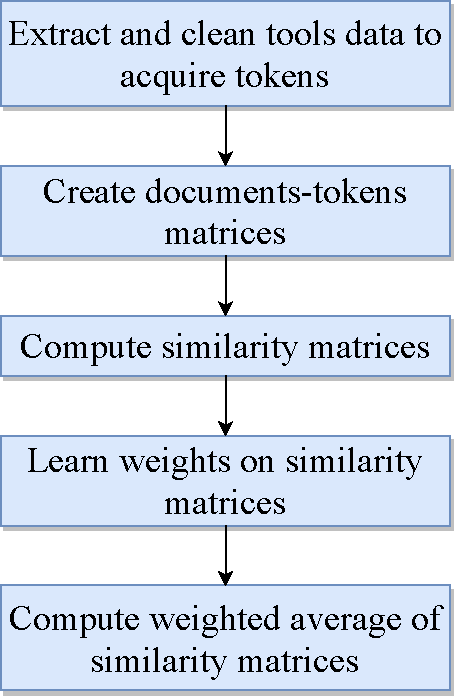
\includegraphics[scale=0.7]{figures/tool_sim_flow.pdf}}
    \caption[Tool similarity flowchart]{\textbf{Sequence of steps to find similar tools}: The image shows a series of steps used to establish similarity among tools using approaches from natural language processing to compute text similarity scores and optimization to combine these similarity scores.}
\end{centering}
\end{figure}

\section{Extract tools data}    
There are multiple repositories of Galaxy tools stored at GitHub \footnote{One example:\url{https://github.com/galaxyproject/tools-iuc/tree/master/tools}}. In each of the tool repository, there are $xml$ files starting with a $<tool>$ tag. We read all of these $xml$ files, extract information from a few of the attributes and collect them in a $tabular$ file.
    
\subsection{Select tools attributes}
A tool has multiple attributes like input and output file types, help text, name, description, citations and some more. But all of these attributes are not important and do not generally identify a tool exclusively. We consider some of these attributes:
\begin{itemize}
	\item Input and output file types
	\item Name and description
	\item Help text
\end{itemize}
Moreover, we combine the input and output file types and name and description respectively as they are of similar nature. These two combined attributes give complete information about a tool file types and its functionality. We also consider help text attribute which is larger in size compared to the previous two. At the same time, they are empty for few tools. Apart from being large in size, this attribute is noisy as well. It provides more information about the usage of a tool. Generally, in the first few lines, it gives a detailed explanation of the tool functions. Further, it explains how the input data should be supplied to a tool or how an input data looks like. Hence, much of the information present in this attribute is not important. Because of noise present in this attribute, we decide to use only upto first $4$ lines which illustrates the core functionality of the tool. The decision to select only first $4$ lines is empirical. The rest of the information in help text is discarded. 


\subsection{Clean tools data}
\subsubsection{Remove duplicates and stopwords}
    The collected data for tools is raw containing lots of commonplace and duplicate items which do not add value. These items should be removed to get $tokens$ which are unique and useful. For example, a tool $bamleftalign$ has input files as $bam, fasta$ and output file as $bam$. While combining the file types, we discard the repeated file types and in this case, we consider file types as $bam, fasta$. The other attributes we deal with are different from the file types. The files types are discrete items but in attributes like name and description and help text, the account is in a human language. The explanation contains complete or partially complete sentences in $English$. Hence, to process this information, we need startegies that are prevalent in natural language processing \footnote{\url{https://www.ncbi.nlm.nih.gov/pmc/articles/PMC3168328/}}. The sentences we write in $English$ contain many words and has different parts. These parts include subject, object, preposition, interjection, verbs, adjectives, adverbs, articles and many others. For our processing, we need only those tokens (words) which categorize a tool uniquely and do away with multiple parts of speech present in the statements. For example, a tool named $tophat$ has name and description as "TopHat for Illumina Find splice junctions using RNA-seq data". The words like $for$, $using$ and $data$ do not give much value as they must be present for many tools. These words are called as "stop words" \footnote{\url{https://www.ranks.nl/stopwords}} and we selectively discard them. In addition, we remove numbers and convert all the tokens to lower case.
  
 
\subsubsection{Use stemming}
After removing duplicates and stop words, our data is clean and contain tokens which uniquely identify corresponding tools. When we frame sentences, we follow grammar which constrains us to use different forms of the same word in varying contexts. For example, a word $regress$ can be used in multiple forms as $regresses$ or $regression$ or $regressed$. They share the same root and point towards the same concept. If many tools use this word in varying forms, it is beneficial to converge all the different forms of a word to one basic form. This is called stemming \footnote{\url{https://nlp.stanford.edu/IR-book/html/htmledition/stemming-and-lemmatization-1.html}}. We use nltk \footnote{\url{http://www.nltk.org/}} package for stemming.

\begin{figure}[h]
\begin{centering}
    {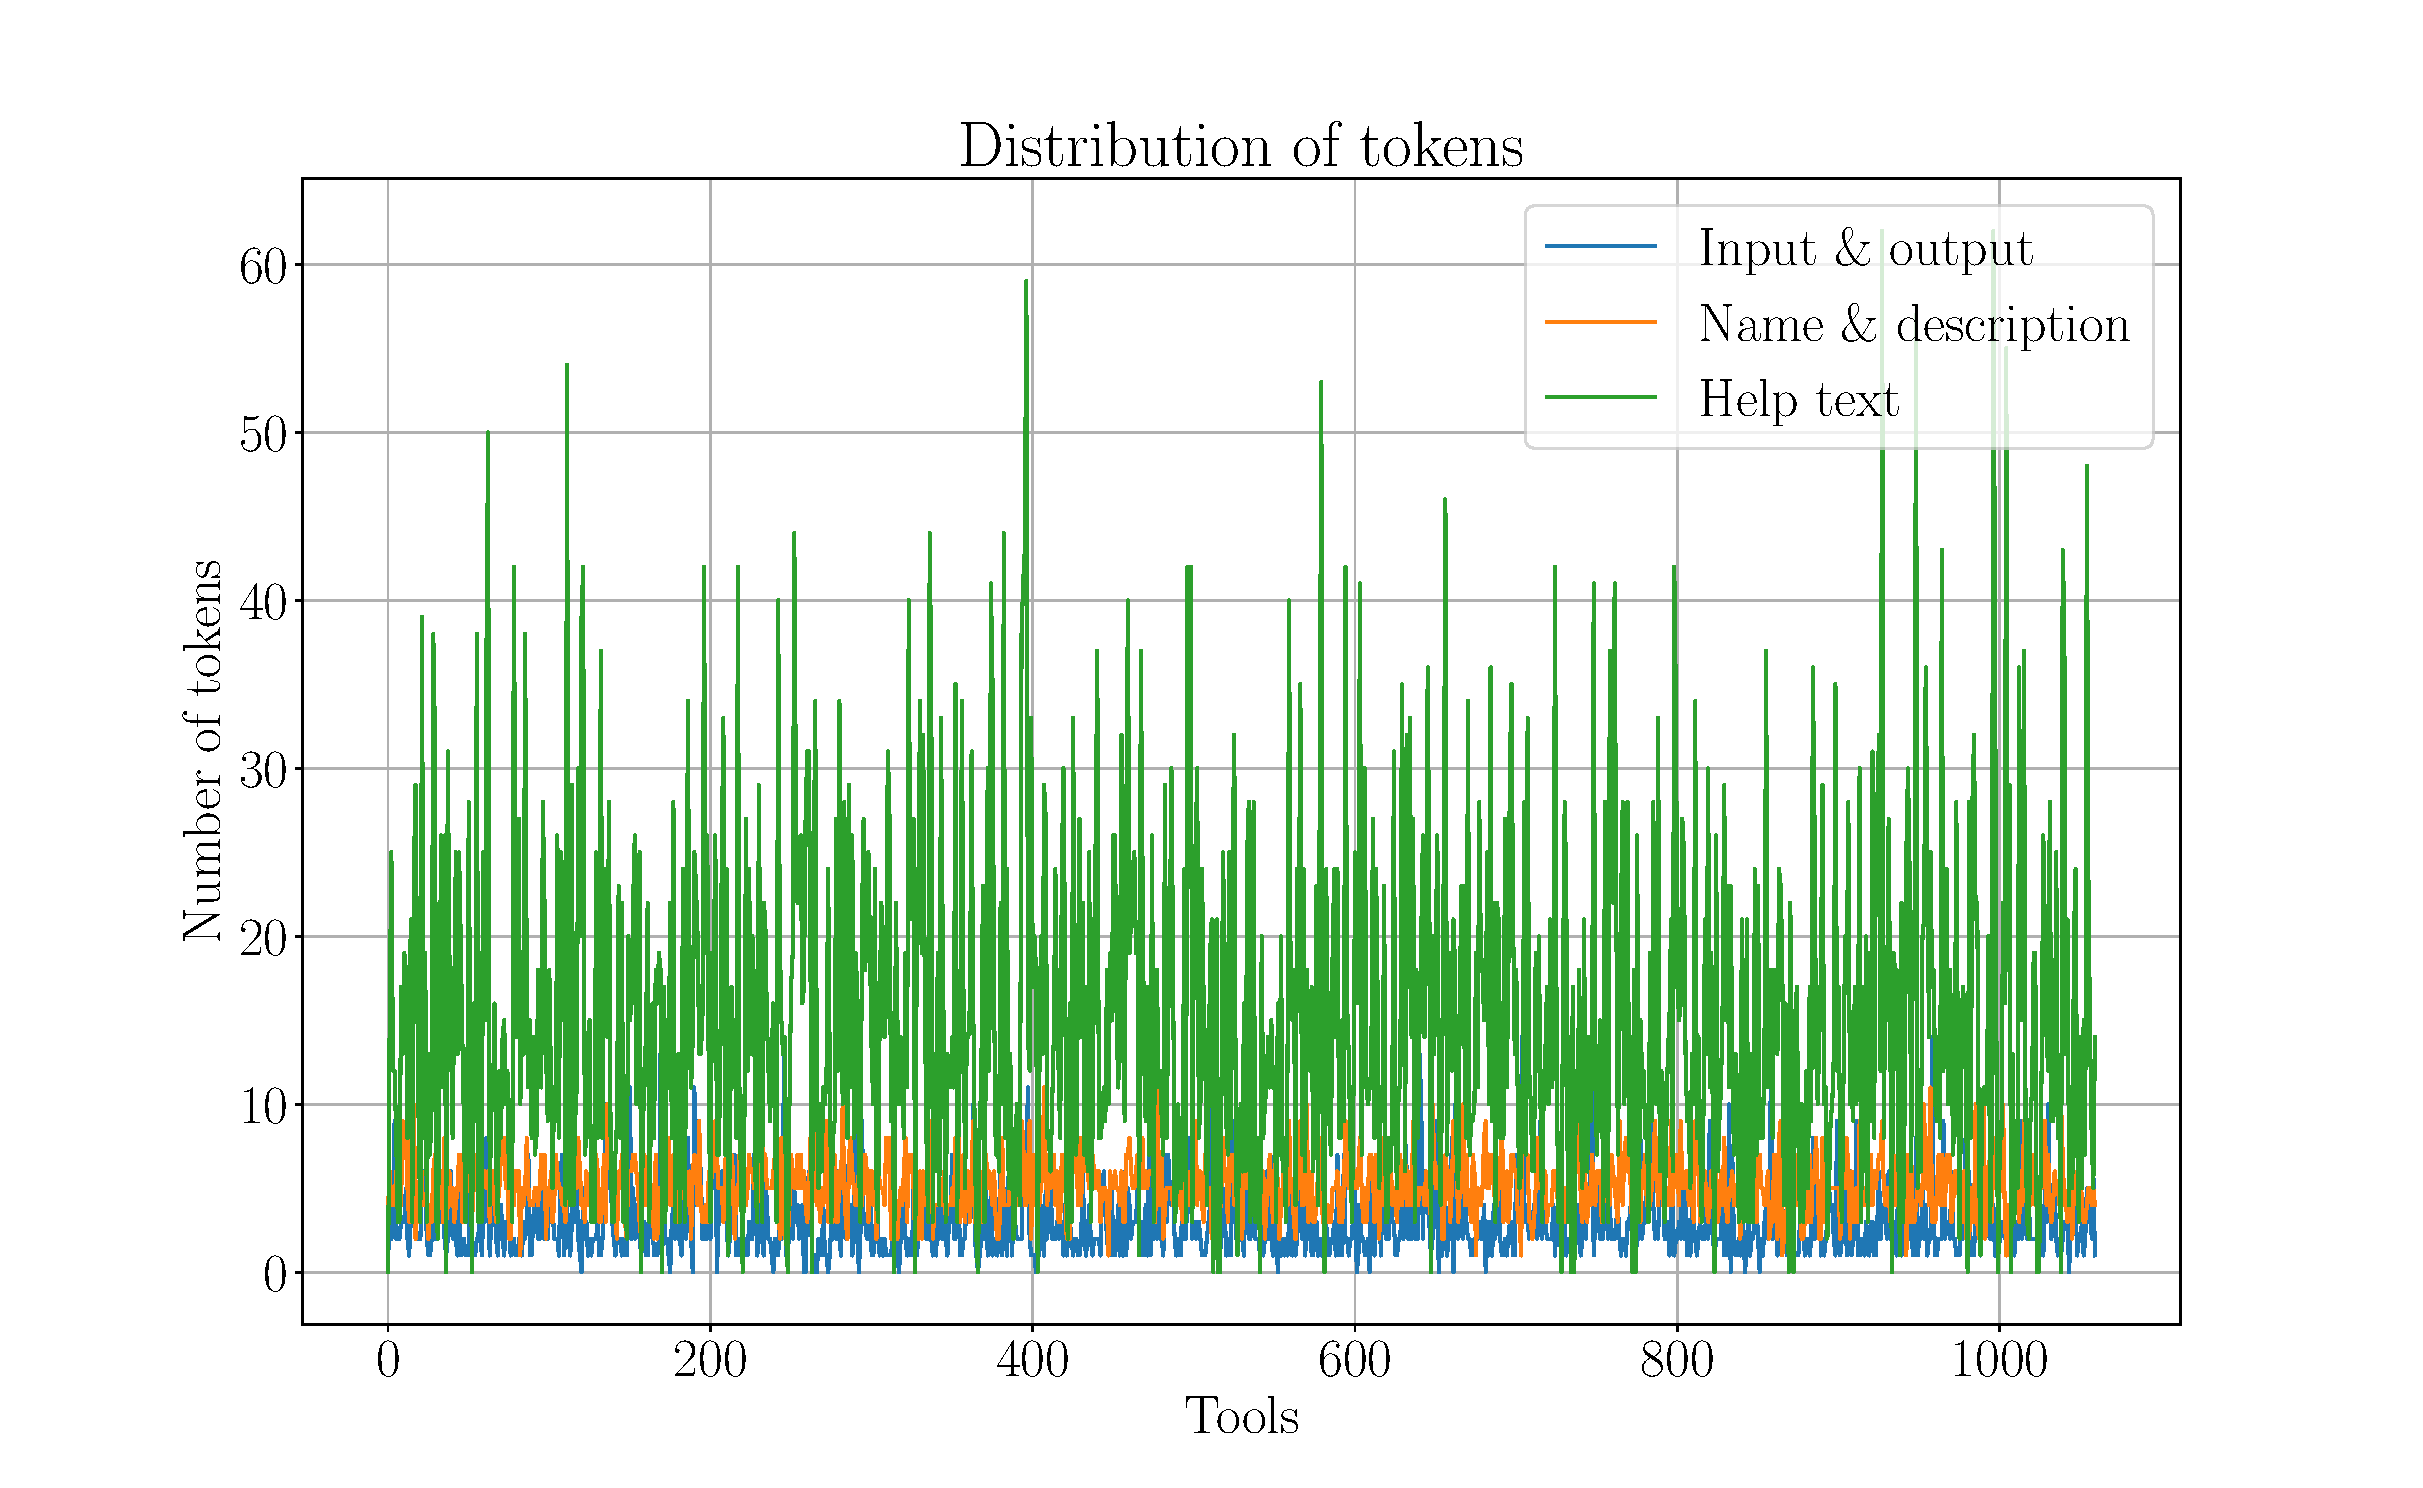
\includegraphics[scale=0.4]{figures/Tokens_dist.pdf}}
    \caption[Tokens distribution]{\textbf{Distribution of tokens (words)}: The plot shows a distribution of tokens for input and output file types, name and description and help text attributes of tools. The help text attribute contains more number of tokens compared to the other two. The input and output file types attribute contains lower number of tokens compared to the other two attributes. }
\end{centering}
\end{figure}

\subsubsection{Learn relevance for words}
    We use a term "token" for each word. For example, a tool's name contains "regress, perform" as a set of tokens (words). After discarding duplicate tokens and stopwords and using root words, we have a set of good tokens for all the three attributes - input and output file types, name and description and help text. Let's call these sets as $documents$. The tokens present in these documents do not carry equal importance. Some tokens are more relevant to the document and some not so relevant . We need to find out importance factor for all tokens in a document. Using these factors, we can arrange them in big, sparse documents-tokens matrix. In this matrix, each row represents a document and each column belongs to one token. To compute these relevance scores, we use bestmatch25. Let's associate some variables to be used in explaining this algorithm.

\begin{figure}[h]
\begin{centering}
    {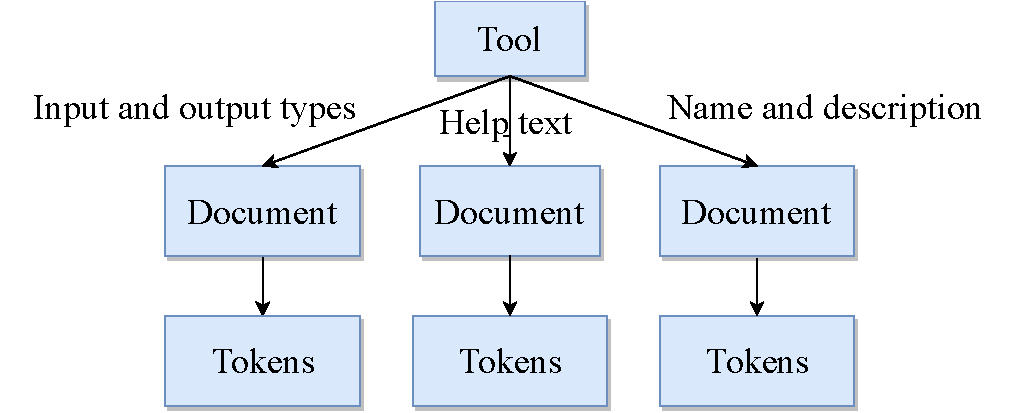
\includegraphics[scale=0.7]{figures/tool-document-tokens.pdf}}
    \caption[Tool, document and tokens]{\textbf{Relationship between a tool, its documents and their tokens}: The image shows that a tool has three documents corresponding to each attribute and each document contains tokens. For all the tools, we have documents equal to the number of tools for each attribute. The number of tokens in each document varies. Minimum number of tokens for any document can be 0.}
\end{centering}
\end{figure}
    \begin{itemize}
	\item Token frequency \footnote{\url{https://nlp.stanford.edu/IR-book/pdf/06vect.pdf}} $tf$
	\item Inverted document frequency $idf$
	\item Average document length $|D|_{avg}$
	\item Number of documents $N$
	\item Size of a document $|D|$
\end{itemize}
    
First of all, token frequency ($tf$) specifies the count of a token's occurrence in a document. If a token $regress$ appears twice in a document, its $tf$ is $2$. This can also be understood as a weight given to this term. Inverted document frequency for a token is defined as:

\begin{equation}
idf = \log \frac{N}{df}
\end{equation}
 
where $df$ is the count of the documents in which this token is present and $N$ is the total number of documents. If we randomly sample a document, then the probability of this token to be present in this document is $ p_i = \frac{df}{N} $. From information theory, we can say that the information contained by this event is $ - \log p_i $. The entity $idf$ is higher when a token appears less number of documents which means that this token is a good candidate for representing the document and possesses higher power to distinguish between documents. The tokens which appear in many documents are not good representatives. Average document length is the average number tokens for all the documents. Size of a document is the count of all the tokens for that document \cite{Robertson:2009:PRF:1704809.1704810}. 


\begin{equation}
\alpha = (1-b) + \frac{b \cdot |D|}{|D|_{avg}}
\end{equation}

\begin{equation}
tf^* = tf \cdot \frac{k+1}{k \cdot \alpha + tf}
\end{equation}

\begin{equation}
BM25_{score} =tf^* \cdot idf
\end{equation}

where $k$ and $b$ are hyperparameters. Using the equation $4$, we compute the relevance score for each token in all the documents. Table 1 shows some sample scores for a few documents where the tokens are present with their respective relevance scores. In this way, we arrange document-tokens matrix for all the attributes of tools. For input and output file types, these matrix entries will have only two value, $1$ if a token is present for a document and $0$ if not. For other attributes, relevance scores are positive real numbers. This strategy of representing documents with their tokens is called vector space model as each document represents a vector of tokens.

\begin{table}[ht]
\begin{center}
    \begin{tabular}{|l|l|l|l|l|l|}
        \hline
        Documents/tokens   & regress & linear & gap & mapper & perform \\ \hline
        LinearRegression   & 5.22 & 4.1 & 0.0 & 0.0  & 3.84 \\ \hline
        LogisticRegression & 3.54 & 0.0 & 0.0 & 0.0  & 2.61 \\ \hline
        Tophat2            & 0.0  & 0.0 & 1.2 & 1.47 & 0.0 \\ \hline
        Hisat              & 0.0  & 0.0 & 0.0 & 0.0  & 0.0 \\ \hline
    \end{tabular}
    \end{center}
    \caption[A sparse documents-tokens matrix]{\textbf{A sparse documents-tokens matrix}: This table shows a matrix of tools (documents) arranged along the rows and tokens along the columns. Each value in the matrix is a weight (relevance-factor) assigned to a token for a document. This matrix is sparse containing mostly zeros as the number of tokens is significantly large compared to the number of tokens present in a doucment. This table shows a sample of how actual documents-tokens matrix would look like.}
    \label{tab:accuracy}
\end{table}

Figure 4 shows the heatmaps for documents-tokens matrices that belong to input and output file types and name and description. We can see that these plots are sparse. Each entry in these matrices contain BM25 score for each token in every document. The representation shows how to find tokens which are good representatives of documents with a weighted by their relevance factors. But, they do not tell un anything about the co-occurence of a few tokens in a document. It tells us that a token is important for a document if the BM25 score is higher but it does not tell us anything about its relation to other tokens. Due to this shortcoming, it does not acknowledge the presence of "concepts" or "context" hidden in a document. A concept in document can be realised when we see the relation among a few words. To illustrate this idea, let's take an example of three words - "New York City". These three words mean little or point to different things if looked at separately. But, if we see them together, it points towards a concept. This vector space model lacks the ability to find the correlation among tokens. To enable the vector space model to learn this hidden concepts and find correlation among multiple tokens, we explore two ideas
\begin{itemize}
\item Latent Semantic Indexing/Analysis \footnote{\url{http://lsa.colorado.edu/papers/dp1.LSAintro.pdf}}
\item Paragraph Vectors
\end{itemize}

Using these approaches, we learn dense, $n$ dimensional vector for each document instead of using sparse vectors as shown in figure 5. 


\begin{figure}[h]
\begin{centering}
    {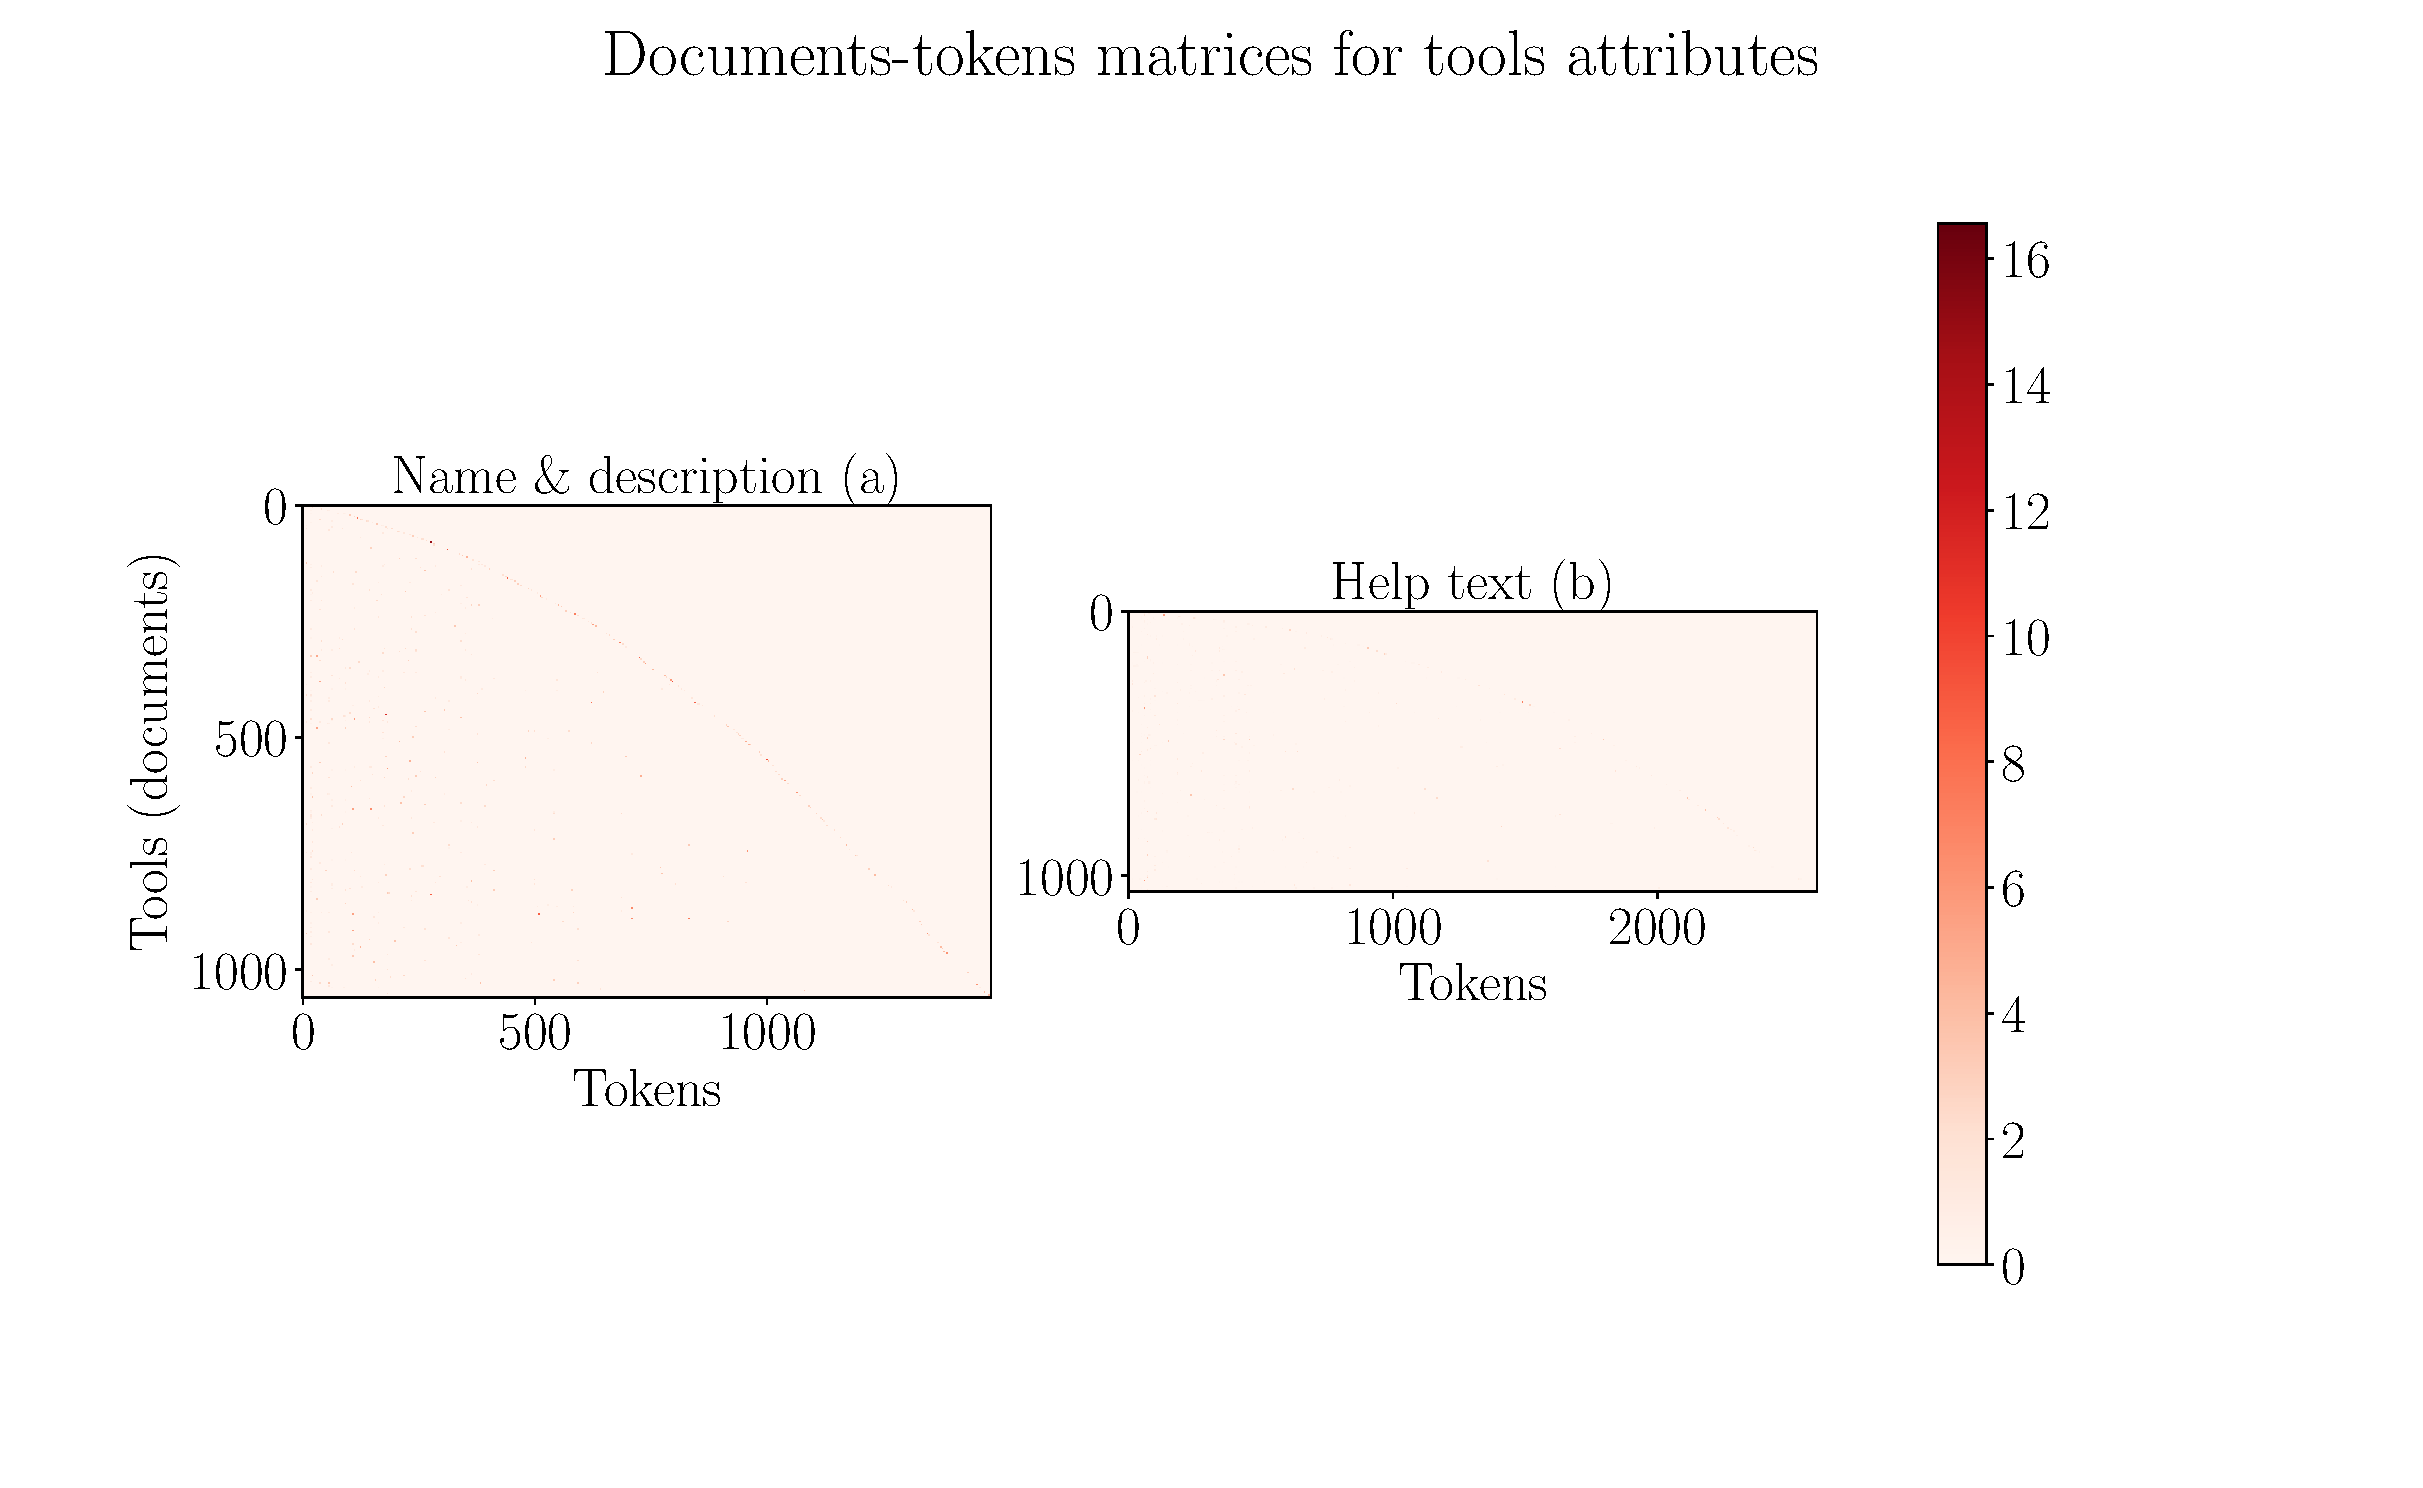
\includegraphics[scale=0.4]{figures/Document_tokens_full_rank.pdf}}
    \caption[Heatmap for documents-tokens matrices]{\textbf{Heatmap for documents-tokens matrices}: The plot shows a heatmap of documents-tokens matrices for name and description and help text attributes. We see that the matrices are sparse containing only few darker spots. The help text matrix is more sparse than name and description matrix as the former contains more number of tokens. We exclude the documents-tokens matrix of input and output file types because we use it as such. For the other two matrices, we would estimate their dense, lower-rank approximations.}
\end{centering}
\end{figure}

    
\section{Learn dense vector for a document}
\subsection{Latent semantic indexing}
    It is a mathematical way to learn the hidden (latent) concepts in documents by computing a low-rank representation of a documents-tokens matrix \cite{Foltz1996, Shapiro2000, Landauer1998}. This low-rank matrix is dense (figure 6). We use singular value decomposition ($SVD$) to decompose the full-rank matrix into a significantly lower rank matrix. The optimal rank to which a matrix to be decomposed is empirical in nature. We would choose ranks from higher to lower value and consequently the sum of singular values would also decrease with the rank. This decomposition follows the equation:
    
    \begin{equation}
    X_{n \times m} = U_{n \times n} \cdot S_{n \times m} \cdot V_{m \times m}^T
    \end{equation}
    
    where $n$ is the number of documents and $m$ is the number of tokens. $S$ is a diagonal matrix containing the singular values in descending order. It contains the weights of the concepts present in the matrix. The matrices $U$ and $V$ and orthogonal matrices which satisfy:
    
    \begin{equation}
    U^T \cdot U = I_{n \times n}
    \end{equation}
    \begin{equation}
    V^T \cdot V = I_{m \times m}
    \end{equation}
    
\begin{figure}[h]
\begin{centering}
    {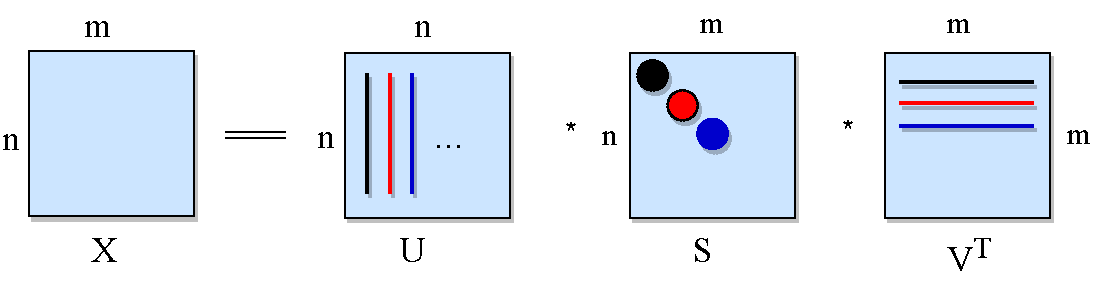
\includegraphics[scale=0.7]{figures/usv.pdf}}
    \caption[Pictorial representation of singular value decomposition]{\textbf{Singular value decomposition}: The image shows that how a matrix is decomposed using singular value decomposition. A matrix $X$ is decomposed into three factor matrices, $U$, $S$ and $V$. The $k$ most important dimensions are kept and the rest are discarded. The value of $k$ is empirical and can be estimated using optimization taking frobenius norm as an error function.}
\end{centering}
\end{figure}

Figure 6 explains \footnote{\url{http://theory.stanford.edu/~tim/s15/l/l9.pdf}} how $SVD$ of a matrix is carried out. The matrix $U$ contains information about how the tokens, arraged along the columns, are mapped to concepts and matrix $V$ stores information about how the concepts are mapped to documents arranged along the rows. 


\subsubsection{Low-rank approximation}
The low-rank approximation of a matrix is important to discard the features which are non-repeating or noise. Using this, we can collect the latent relations present in the documents-tokens matrices. We saw that our documents-tokens matrices suffer from sparseness and exhibit no relation among tokens. The approximation deals with these issues as well. The resulting matrices are dense and contain most of the singular values. The singular values which are small (the last entries of the $s$ matrix along the diagonal) are discarded \cite{DBLP:journals/corr/Yang15b}. The low-rank approximated matrix $X_k$ is computed as:
    \begin{equation}
    X_{n \times m} = U_{k} \cdot S_{k} \cdot V_{k}^T
    \end{equation}
    where $U_{k}$ is the first $k$ columns of $U$, $V_{k}$ is the first $k$ rows and $S$ is the first $k$ singular values. $k$ is an empirical parameter. $X_k$ is called as the rank-k approximation of the full rank matrix $X$. Figure 7 shows the variation of the sum of singular values with the percentage rank of matrices. The percentage rank is $k \div K$ where $1 <= k <= K$ and $K$ is the original (full) rank of a matrix. We take it as the original ranks of the three matrices are not comparable. By doing this, we can show them on one plot. Similar idea we use for the sum of the singular values of each matrix. From figure 7, we can say that if we reduce the ranks of matrices to $70\%$ of the full-rank, we can still capture $\approx 90\%$ of the singular values. The reduction to half of the full-rank achieves $\approx 80\%$ of the sum of singular values. 

\begin{figure}[h]
\begin{centering}
    {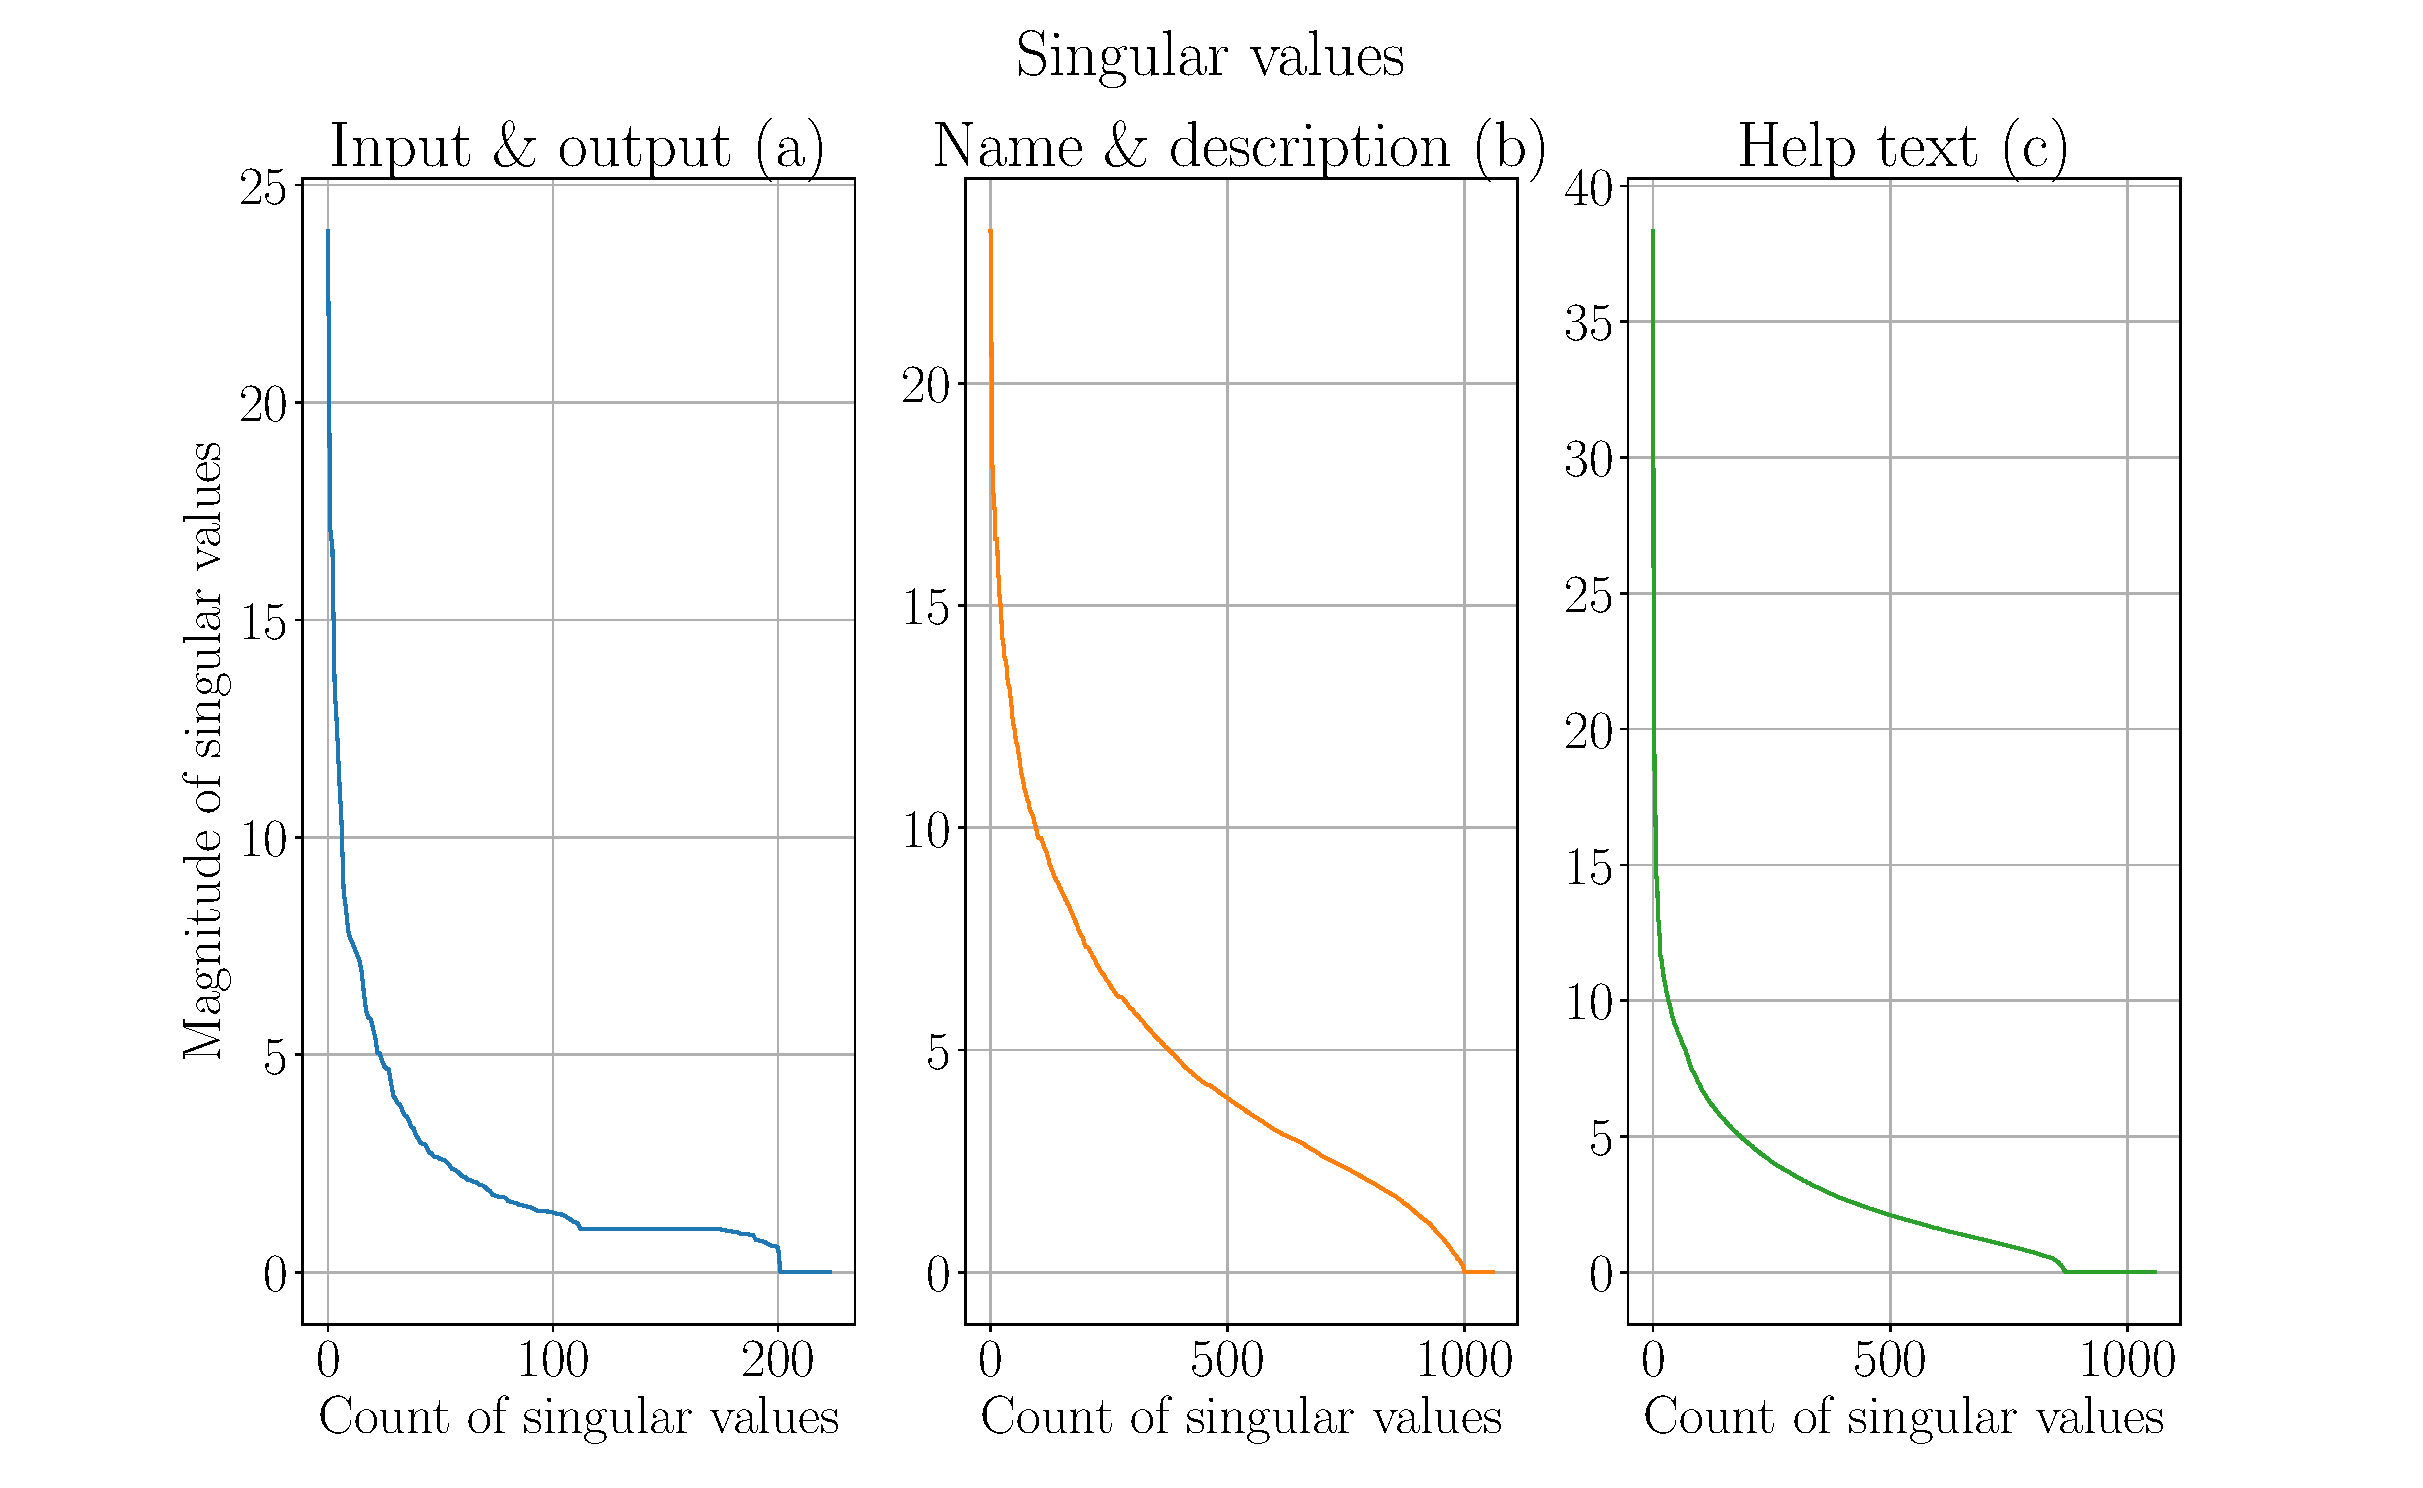
\includegraphics[scale=0.35]{figures/Singular_values.pdf}}
    \caption[Singular values of documents-tokens matrices]{\textbf{Singular values of the documents-tokens matrices}: The plot shows singular values computed using singular value decomposition (equation 5). The diagonal matrix $S$ contains these singular values sorted in descending order. We can see that in (a), (b) and (c) that very few singular values have higher mangnitude and most of the singular values are smaller. }
\end{centering}
\end{figure}

\begin{figure}[h]
\begin{centering}
    {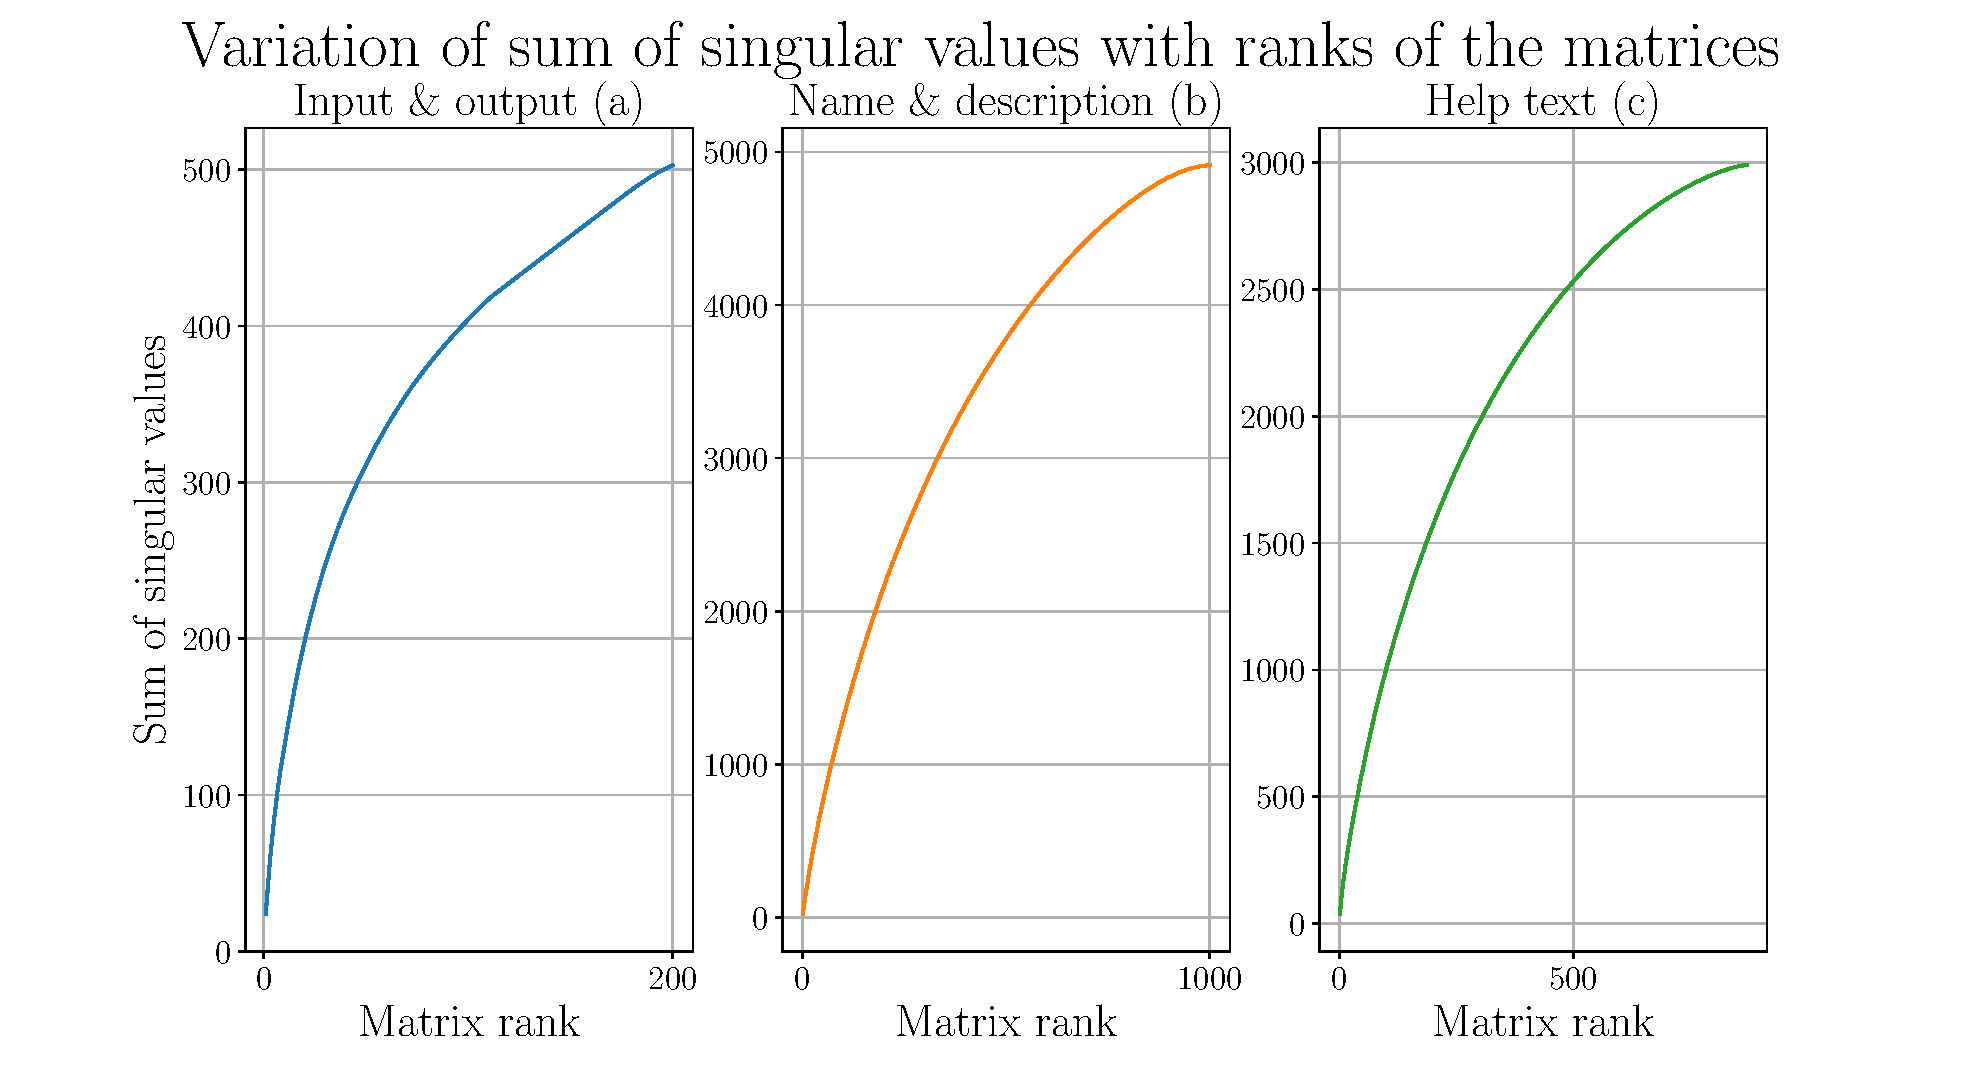
\includegraphics[scale=0.45]{figures/Sum_singular_ranks.pdf}}
    \caption[Singular values of documents-tokens matrices with their respective ranks]{\textbf{Sum of singular values with matrix rank}: The plot shows an easier way to see how the sum of singular values varies with a documents-tokens matrix rank for the three attributes. Here the (a), (b) and (c) show separately this variation as the ranks of these matrices and sum of singular values differ.}
\end{centering}
\end{figure}

\begin{figure}[h]
\begin{centering}
    {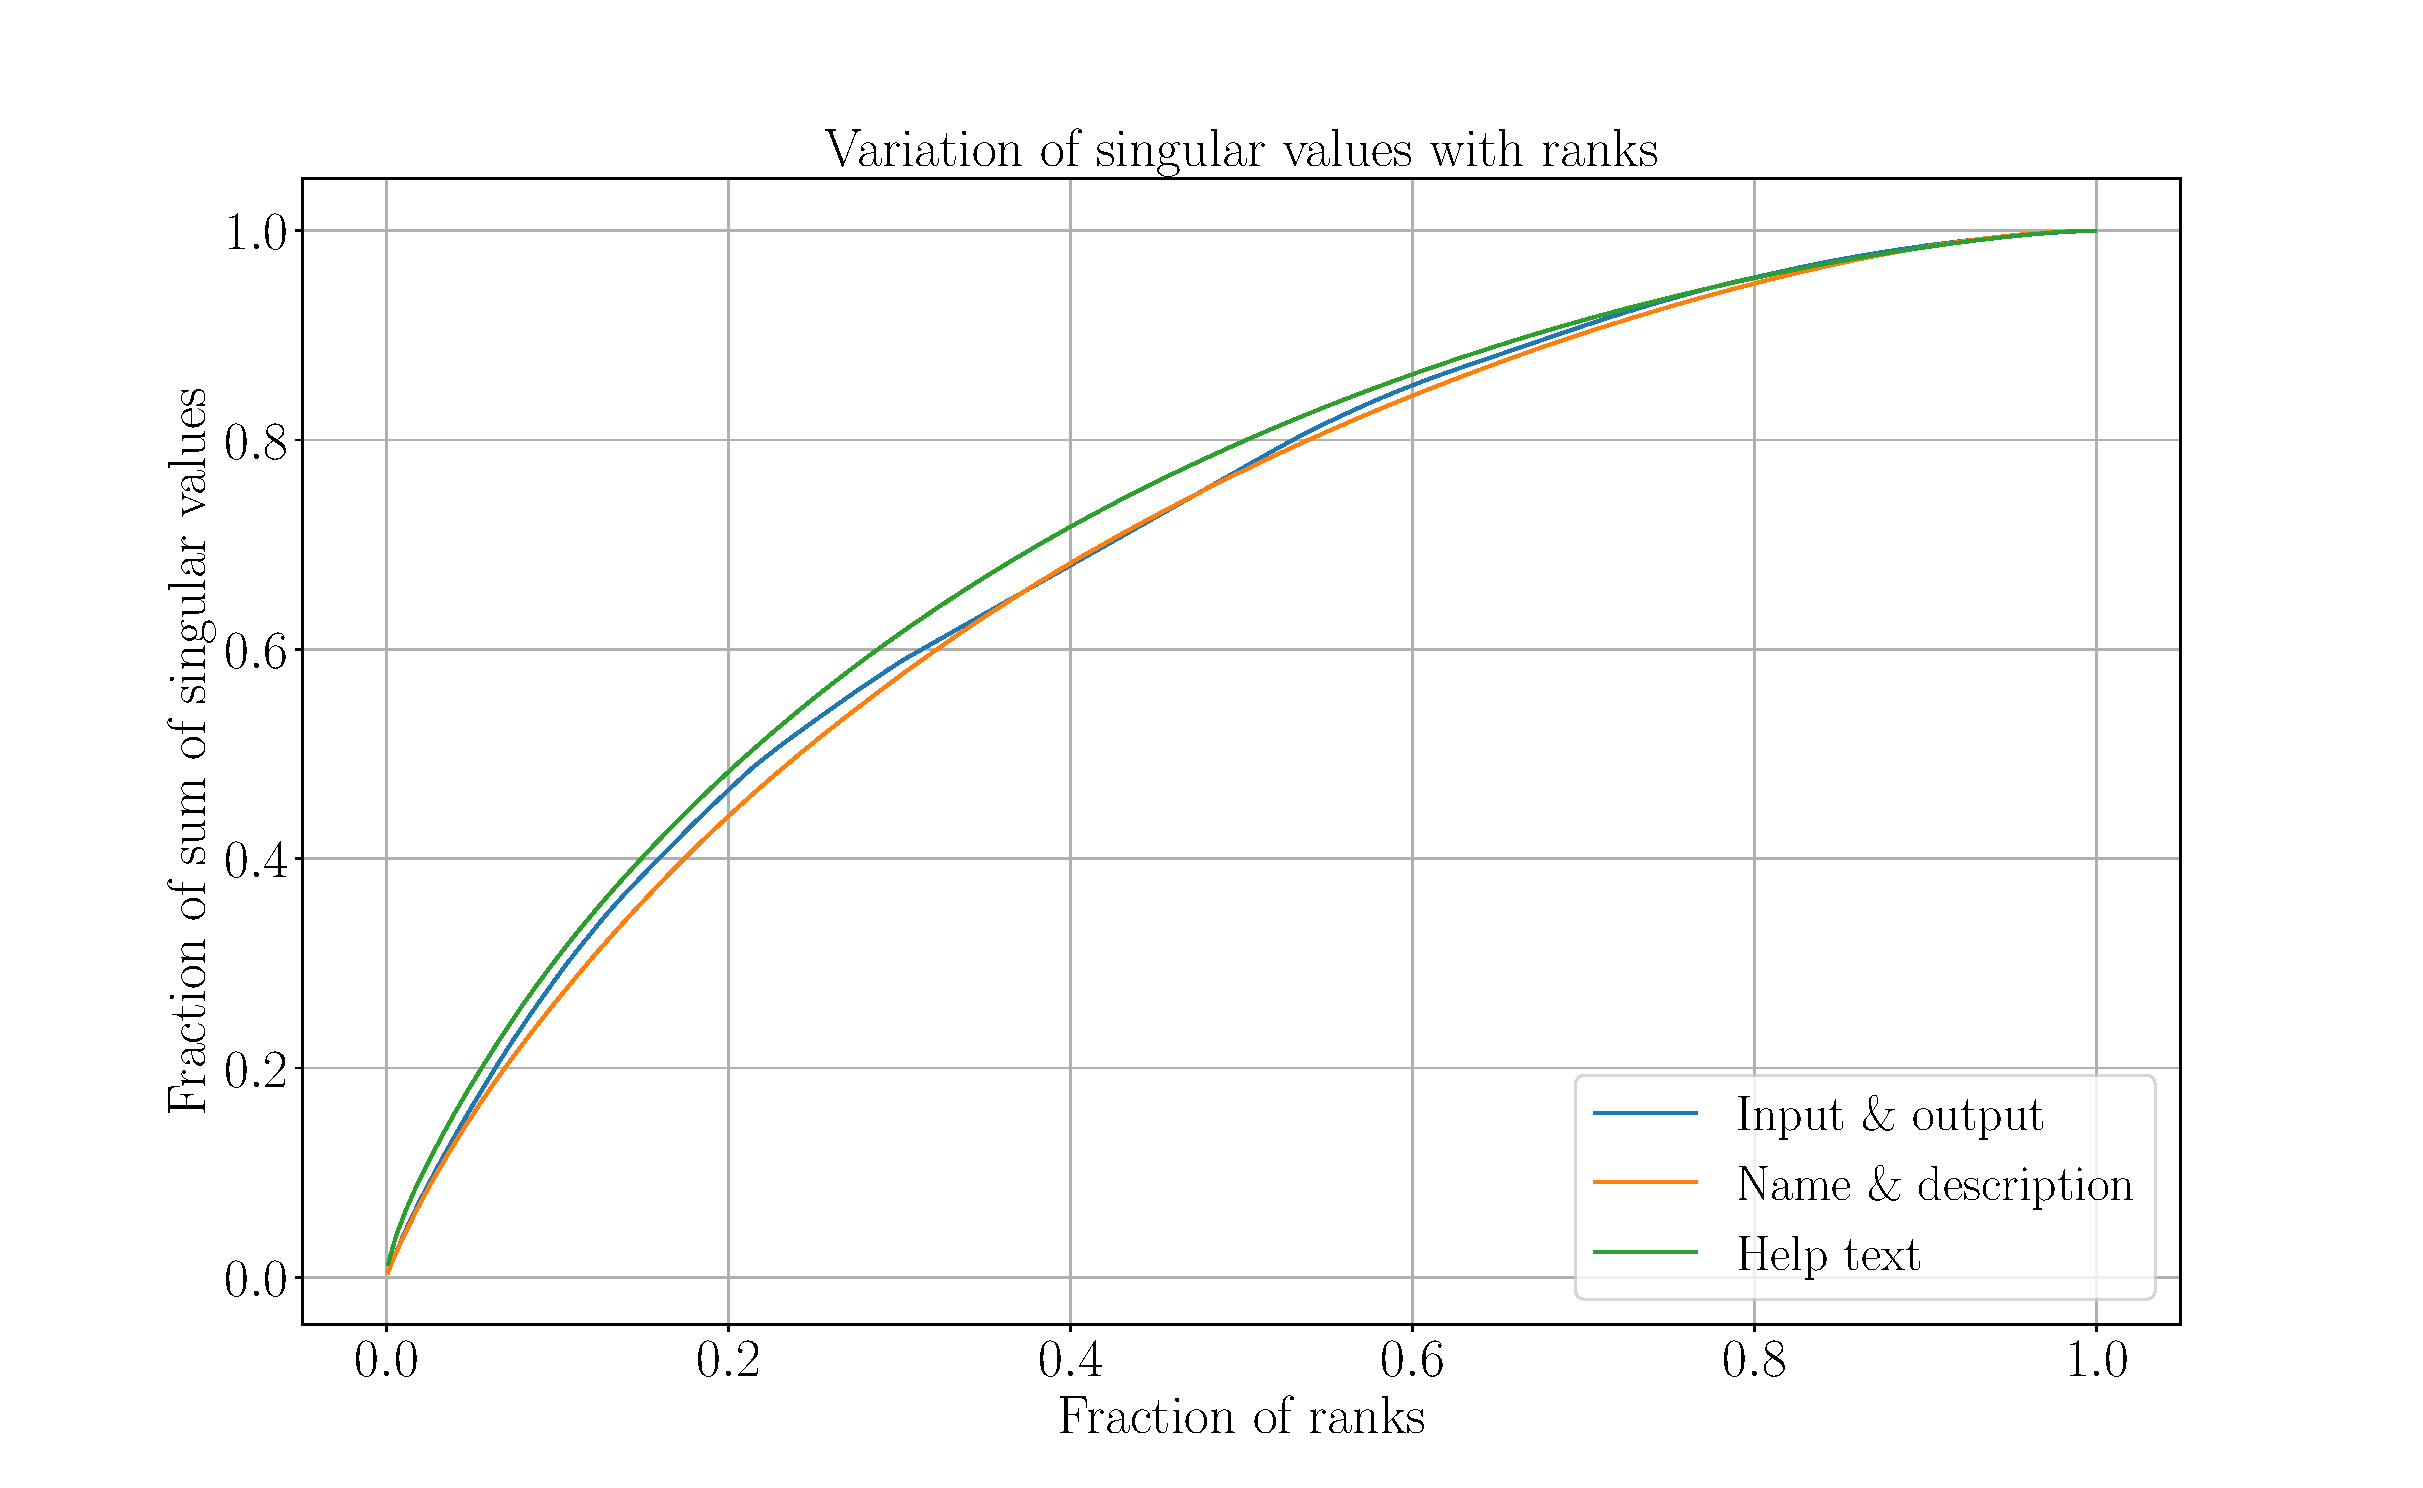
\includegraphics[scale=0.4]{figures/Fraction_ranks_singular_values.pdf}}
    \caption[Fraction of ranks of documents-tokens matrices with the fraction of sum of singular values]{\textbf{Fraction of ranks of documents-tokens matrices with the fraction of sum of singular values}: This plot merges the results of the figure 10 into one plot. As the ranks of document-term matrices and sum of singular values vary, we convert them to respective percentages. $rank_{fraction} = \frac{k}{N}$ where $k$ is the reduced rank and $N$ is the full-rank of a matrix For example $0.2$ on the rank axis (x-axis) means $20\%$ of the original rank of a matrix. Similarly, y-axis shows the fraction of the sum of all singular values $ sum_{fraction} = \frac{\sum_{i=1}^k}{\sum_{i=1}^K}$ where $K$ is the number of all singular values.}
\end{centering}
\end{figure}

We reduce the rank of the original documents-tokens matrices and compute the dense and approximated low-rank matrices. Figure 8 shows the low-rank matrices for input and output file types and name and description attributes. For computing this, we use only $40\%$ of the full-rank. We can compare it with figure 5 and deduce that figure 8 is denser than figure 5. In these low-rank matrices, we have dense vector representations for documents along the rows. In each matrix, each row contains a vector for one document. Using these documents vectors, we can compute the correlation or similarity using any similarity measure. There are multiple similarity measures that can be used like euclidean distance, cosine similarity, manhattan distance. We use cosine angle similarity to compute the correlation between vectors. By this, we get a positive real number between $0.0$ and $1.0$ specifying how similar a pair of documents are. The higher the score, higher is the similarity. Computing this similarity for all the documents give us a similarity matrix $S_{n \times n}$ where $n$ is the number of documents. This square, symmetric matrix is called as similarity or correlation matrix. We compute three such matrices each corresponding to one attribute.
  
\begin{figure}[h]
\begin{centering}
    {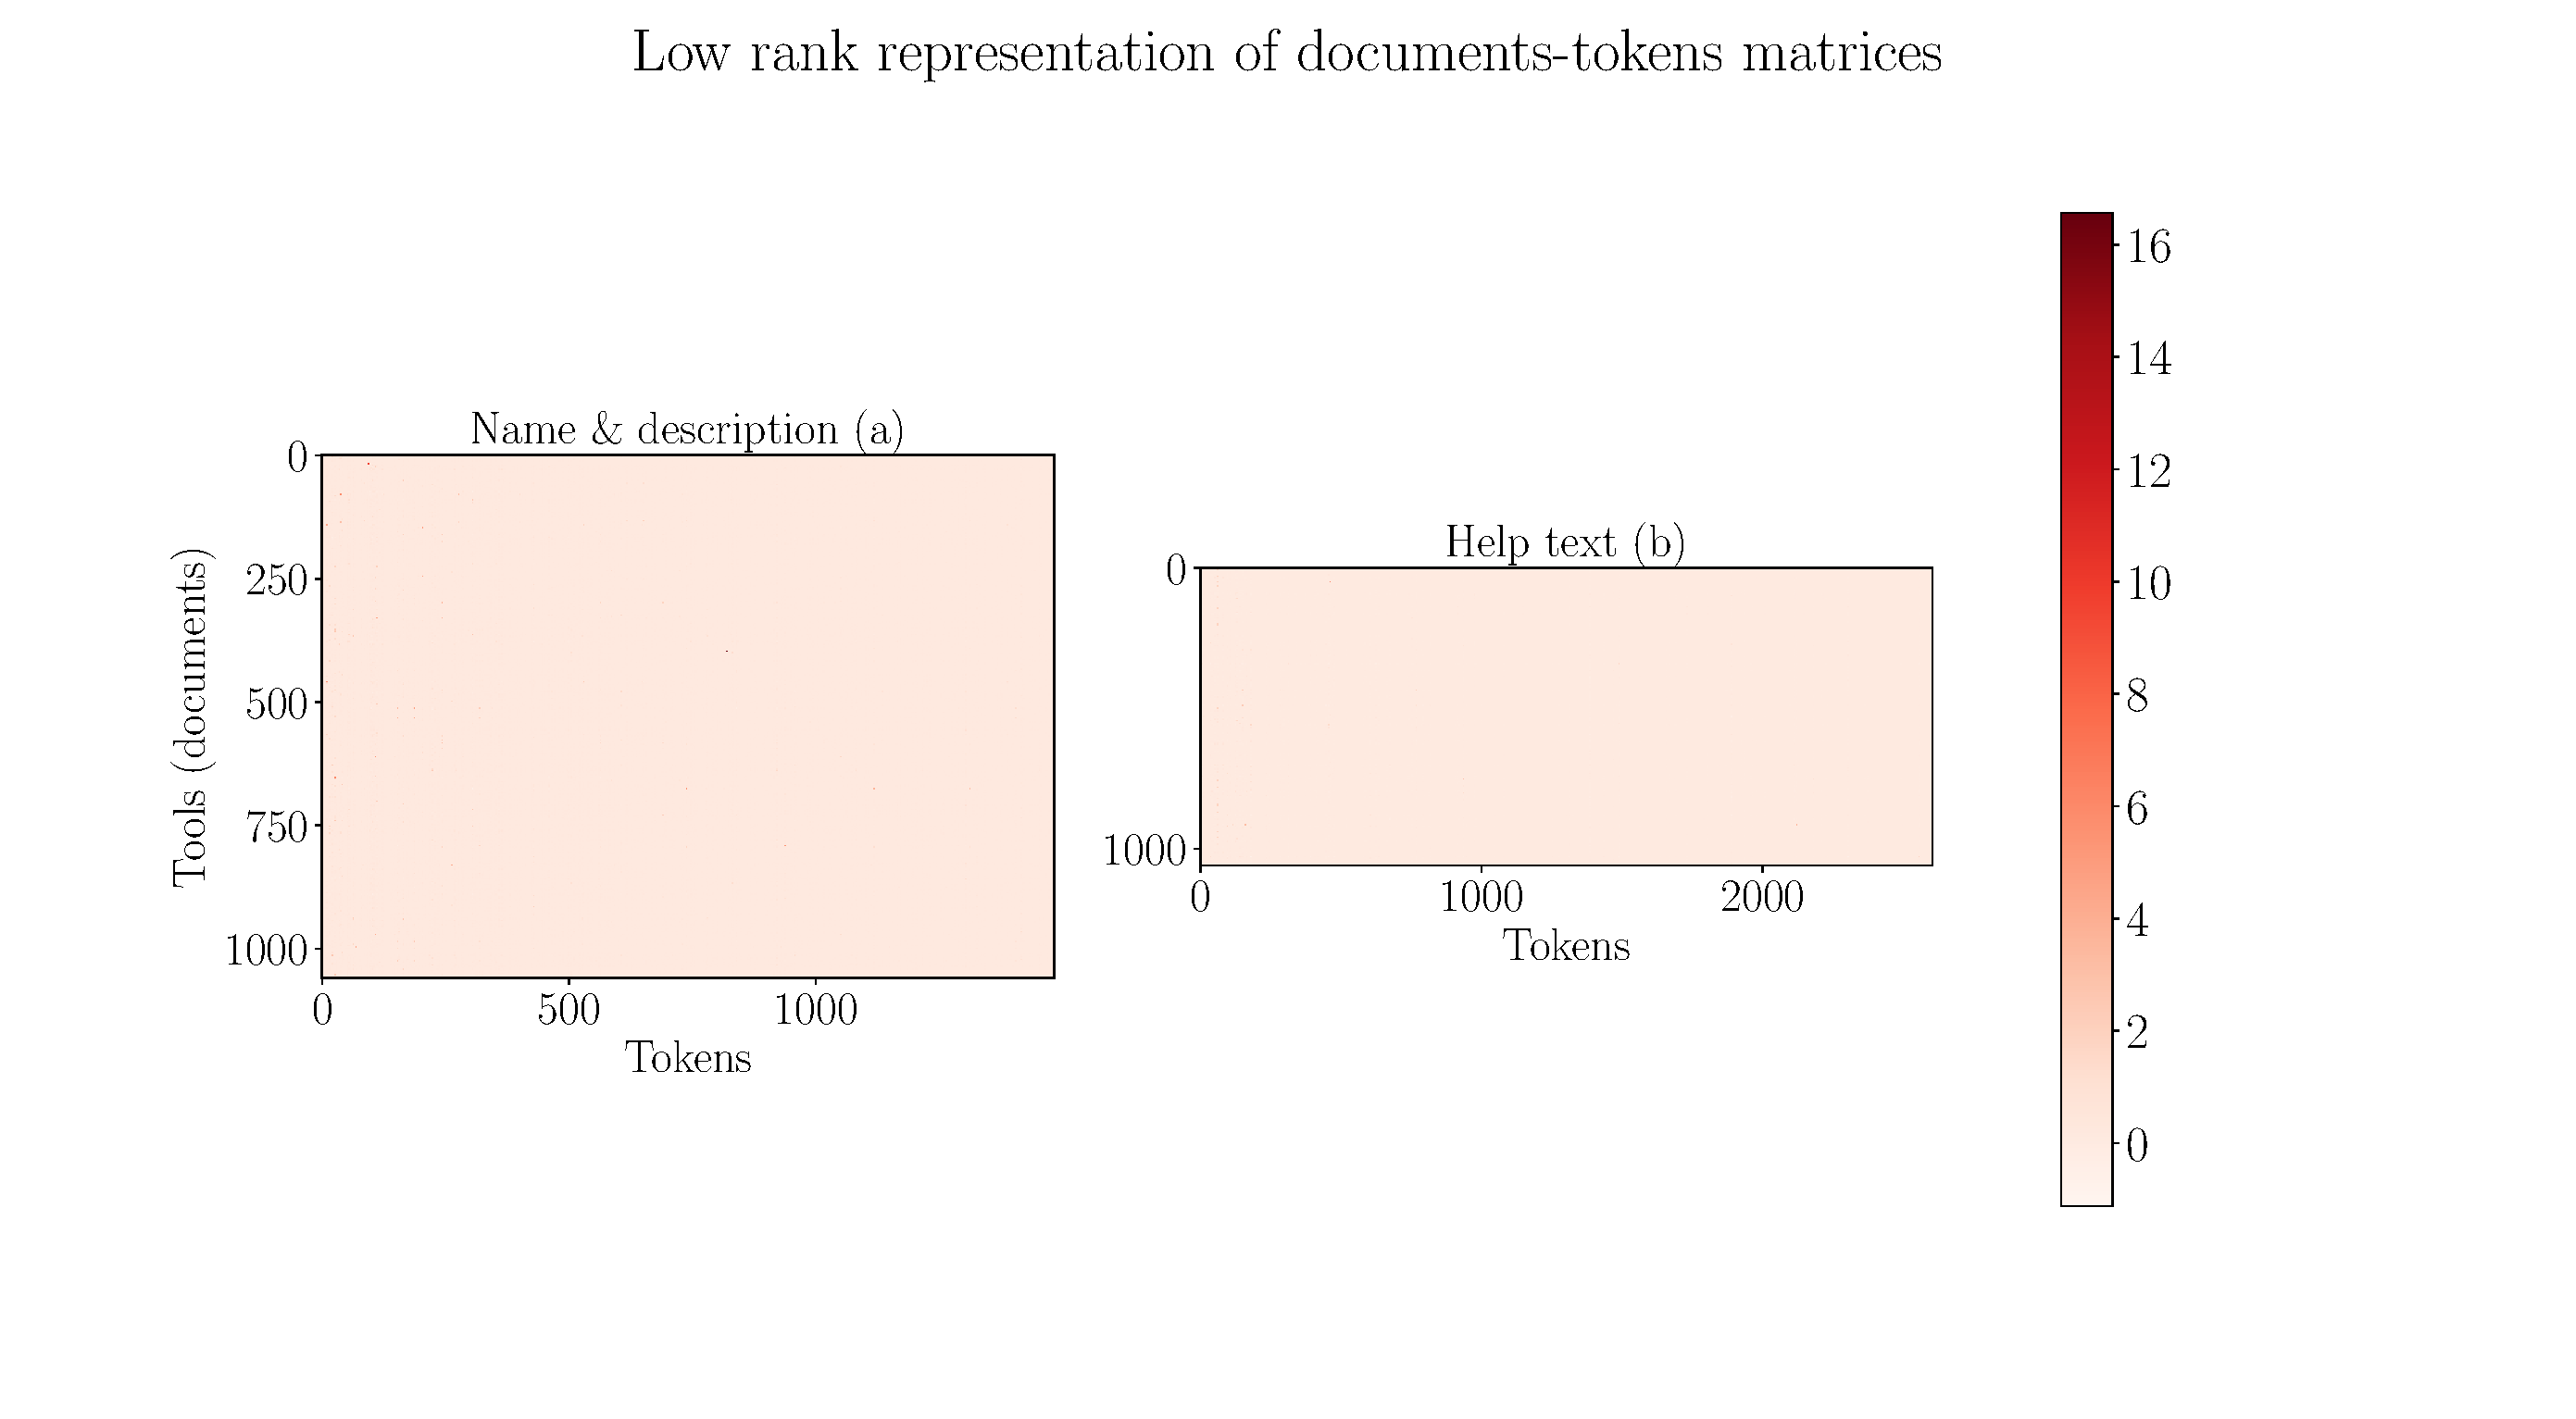
\includegraphics[scale=0.35]{figures/Document_tokens_low_rank.pdf}}
    \caption[Low-rank representations of documents-tokens matrices]{\textbf{Low-rank representations of documents-tokens matrices}: The heatmap shows the low-rank ($5\%$ of full-rank) representations of documents-tokens matrices for name and description and help text. These matrices are more dense compared to figure 7 which shows these matrices corresponding to the full-rank representations.}
\end{centering}
\end{figure}

\subsection{Paragraph vectors}
Using latent semantic indexing (LSI), we learnt dense vectors to represent each document. It learns better vector representations for documents compared to using full-rank documents-tokens matrices. One main limitation is to assess the quantity by which we need to lower the rank of a matrix in order to find the optimal results. There are ways to find the optimal reduced rank optimizing the frobenius norm but it is not simple. We would see in the analysis section that similar tools are more dominated by the scores shared by the input and output file types due to which the tools which similar in their functions do not come up. In order to avoid these limitations, we use an approach known as $doc2vec$ (document to vector). It learns a dense, fixed-size vectors for each document using neural networks. These vectors are unique in a way that captures the semantics present in the documents. The documents which share similar context are represented by similar vectors. When we compute cosine distance between these vectors sharing similar context, we get a higher number (close to 1.0). It allows the documents to have variable lengths.


\subsubsection{Approach}
Paragraph vectors approach learns vector representations for all the words present in a set of documents. The words which are used in a similar context have similar vectors. For example, words like "data" and "dataset" which are used, in general, in similar context have are represented by close vectors. The vector representations of words in a corpus is learnt by finding the maximum of the following equation:

\begin{equation}
\frac{1}{T} \cdot \sum_{t=k}^{T-k} \log p(w_t|w_{t-k,...,t+k})
\end{equation}

where $T$ is the total number of words in a corpus, $k$ is the window size. We take a few words which make a context and using this context we try to predict each word. The probability $p$ is computed using a softmax classifier and backpropagation is used to compute the gradient and the vectors are optimized using stochastic gradient descent. To learn paragraph vectors, in addition to using words vectors, paragraph vectors are also used to learn probability of the next words in a context. The paragraph and word vectors are averaged to make the classifier which predict next words in a context. There are two way how to choose the context. 

\begin{itemize}
\item Distributed memory: In this approach of learning paragraph vectors, fixed length window of words are choosen and paragraph vectors and word vectors are used to predict the words in this context. The words vectors are shared across all paragraphs and paragraph vector is unique to each paragraph.

\begin{figure}[h]
\begin{centering}
    {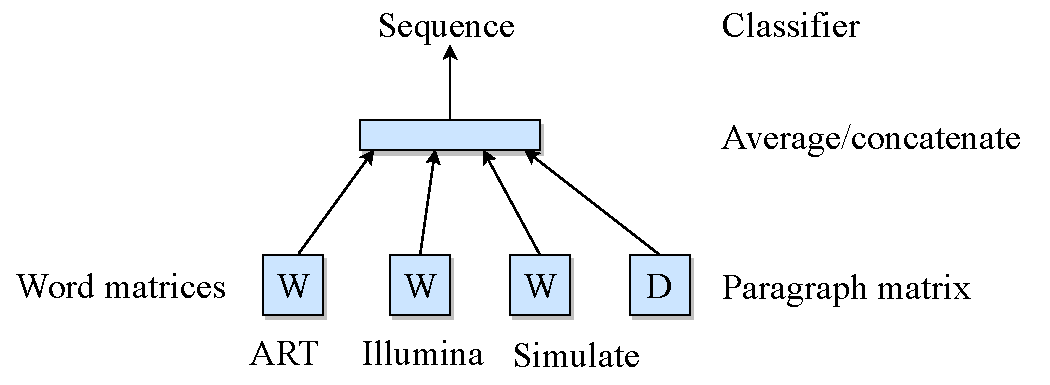
\includegraphics[scale=0.7]{figures/dm_pv.pdf}}
    \caption[Distributed memory approach for paragraph vectors]{\textbf{Distributed memory approach for paragraph vectors}: This image shows the mechanism for learning a vector for a paragraph. $W$ is a word matrix where each word is represented by a vector. $D$ is a paragraph matrix where each paragraph (document) is represented by a vector. The word vectors are shared across all paragraphs (documents) but not the paragraph vectors. The three words "Art", "Illumina" and "Simulate" represent a context. The average or concatenated words and paragraph vectors are used to predict the "Sequence" word.}
\end{centering}
\end{figure}

\item Distributed bag of words: The words are randomly extracted from paragraphs and in this set of words, a word is chosen randomly and predicted using the paragraph vectors. The order of the randomly chosen words is ignored.  
\end{itemize}

\begin{figure}[h]
\begin{centering}
    {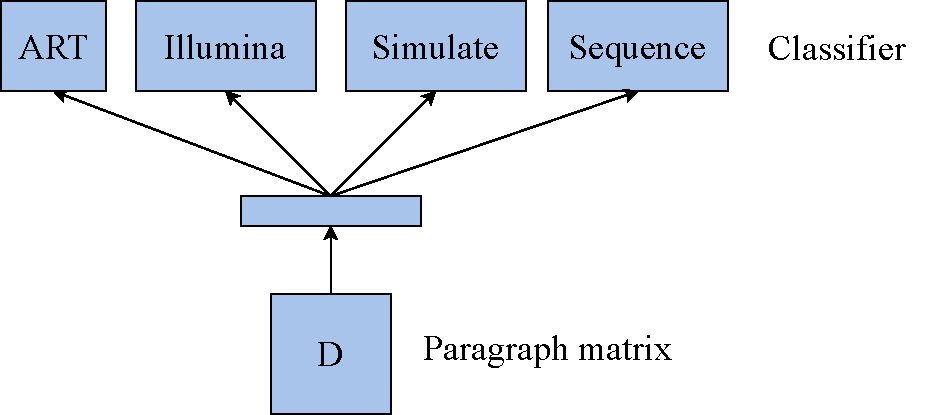
\includegraphics[scale=0.7]{figures/dbow_pv.pdf}}
    \caption[Distributed bag-of-words approach for paragraph vectors]{\textbf{Distributed bag-of-words approach for paragraph vectors}: This image shows how only paragraph vectors are learned by predicting a random word choosen from a randomly selected set of words. In this approach, the order of the words does not matter.}
\end{centering}
\end{figure}

The figures 9 and 10 are inspired from the original work - Distributed Representations of Sentences and Documents \footnote{\label{pv}\url{https://arxiv.org/abs/1405.4053}}.
The second form of learning paragraph vectors is simple and we use it to learn documents (paragraphs) vectors for name and description and help text attributes. We learn only the paragraph vectors which makes it less computationally expensive \cite{DBLP:journals/corr/LeM14}.


\section{Similarity measures}
We have vectors representing the documents for all the three attributes we consider to compute similar tools. To find the similarity in a pair of vectors, we need to apply a similarity measure to get a similarity score. This score quantifies how much similar a pair of documents are which means how close or distant these documents are.


\subsection{Cosine similarity}
It gives the cosine angle value between a pair of documents vectors. Let's say we have two vectors, $x$ and $y$. We can write:
\begin{equation}
x \cdot y = |x| \cdot |y| \cdot \cos{\theta}
\end{equation}

\begin{equation}
\cos{\theta} = \frac {x \cdot y}{|x| \cdot |y|} 
\end{equation}

where $|.|$ is the norm of the vector $x$. If the norm is $0$, we use $0$ for the value of $\cos{\theta}$. The values emitted by this similarity follows a natural progression that if the documents are dissimilar, then it is $0$ and if completely similar, it is $1.0$. Otherwise it lies between $0.0$ and $1.0$. This score can also be understood as a kind of probability of similarity between a pair of documents \footnote{\url{https://nlp.stanford.edu/IR-book/html/htmledition/dot-products-1.html}}. 


\subsection{Jaccard index}
Jaccard index is a measure of similarity between two sets of entities given by the equation:

\begin{equation}
j = \frac{A \cap B}{A \cup B}
\end{equation}
where $A$ and $B$ are two sets. $\cap$ is the number of entities present in both the sets and $\cup$ is the sum of unique entities present in sets $A$ and $B$ \cite{Ivchenko1998}. We use this measure to compute the similarity between two tools based on their file types. For example, $LinearRegression$ has 3 file types: $tabular$, $input$ and $pdf$. Another tool $LDAAnalysis$ has $tabular$ and $txt$ as file types. The jaccard index for this pair of tools would be:

\begin{equation}
j = \frac{Length[(tabular, input, pdf) \cap (tabular, txt)]}{Length[(tabular, input, pdf) \cup (tabular, txt)]}
\end{equation}

\begin{equation}
j = \frac{1}{4} = 0.25
\end{equation}


\section{Optimization}
Using the paragraph vectors and applying cosine similarity, we get similarity or correlation matrices one each for input and output file types, name and description and help text attributes. The matrices have same dimensions ($n \times n$, $n$ is the number of tools). To combine these matrices, one simple idea would be to take an average of the corresponding rows of scores from the matrices for a document. This would generate a matrix of the same dimension where each row would correspond to one document. This row would contain similarity scores of a document against all other documents. The diagonal entries of this matrix would be 1.0. All other entries would be a positive real number between $0.0$ and $1.0$. Another way to find the combination is to learn the weights on the rows from three matrices and them combine them to obtain optimal similarity scores for a tool. The weight would be a positive real number between $0.0$ and $1.0$. Instead of using a fixed importance factor (weights) of $1 / 3$ ($3$ is the number of matrices), we use optimization to find these real numbers and then combine the matrices by multiplying with these weights.

\begin{equation}
S_k^{optimal} = w^k_{io} \cdot S^k_{io} +  w^k_{nd} \cdot S^k_{nd} + w^k_{ht} \cdot S^k_{ht}
\end{equation}

where $w$ is a positive, real number and satisfy $w^k_{io} + w^k_{nd} + w^k_{ht} = 1$. 
$S^k_{io}$, $S^k_{nd}$ and $S^k_{ht}$ are the similarity scores (corresponding matrix rows) for $k^{th}$ tool corresponding to input and output file types, name and description and help text attributes respectively.

We have these similarity scores. But we need to learn these importance weights. We use gradient descent optimizer to learn these weights against a loss function. If we look closely the similarity measure, we see that the maximum similarity between a pair of documents can be $1.0$. Hence, the ideal similarity scores for one document against all other documents:

\begin{equation}
S_{ideal} = [ 1.0, 1.0, ...., 1.0 ]
\end{equation}
where $S_{ideal}$ is the ideal similarity scores for one document against all other document. Using this ideal scores, we can compute the error we accrue for all the similarity scores from three attributes. After computing the error, we can verify which attribute is closer to the ideal score and which are not. The attributes which exhibit lower error get higher weights and those which score higher error get lower weights. The next section elaborates the online way to do the optimization.


\subsection{Gradient descent}
Gradient descent is a popular algorithm for optimizing an objective function with respect to its parameters. The parameters are the entities which we want to learn. In our case, these are the weights. The algorithm minimizes an error function. Let's frame the error function:

\begin{equation}
Error^k_{io}(w_{io}) = \sum_{t=1}^{N-1} \cdot (w_{io} \cdot S^t_{io} - S_{ideal}) ^ 2
\end{equation}

\begin{equation}
Error^k_{nd}(w_{nd}) = \sum_{t=1}^{N-1} \cdot (w_{nd} \cdot S^t_{nd} - S_{ideal}) ^ 2
\end{equation}

\begin{equation}
Error^k_{ht}(w_{ht}) = \sum_{t=1}^{N-1} \cdot (w_{ht} \cdot S^t_{ht} - S_{ideal}) ^ 2
\end{equation}

\begin{equation}
Error^k(w) = \sum_{t=1}^{N-1} \cdot (w \cdot S^t - S_{ideal}) ^ 2
\end{equation}

\begin{equation}
\argmin_w Error^k(w) 
\end{equation} 

where $Error$ is a vector of $<Error_{io}, Error_{nd}, Error_{ht}$,
$w$ is $<w_{io}, w_{nd}, w_{ht}>$ and $S$ is $<S_{io}, S_{nd}, S_{ht}>$.

To minimize the equation $17$, we need to compute the gradient. The gradient specifies the rate of change of error with respect to the weights.

\begin{equation}
Gradient^k(w) = \frac{\partial Error^k}{\partial w} = 2 \cdot \sum_{t=1}^{N-1} (w \cdot S^t - S_{ideal}) \cdot S^t
\end{equation}

Using the gradient vector, we update the weights. For this we need to set the learning rate.

\begin{equation}
w^k = w^k - \eta \cdot {Gradient(w^k)}
\end{equation}

To find the right learning rate is important as a high value can diverge the gradient learning and a low value can slow down the learning. For each iteration of gradient descent, we employ time-based decay of learning rate.


\subsection{Learning rate decay}
To find an optimal learning rate forms an important part of gradient descent optimization. If the learning rate is high, it poses a risk of optimizer divergence. On the other hand, if is small, the optimizer can take a very long time to converge. Both these situations are underisable and we can avoid them by starting out with a small value and gradually decrease the learning rate over iterations. It is called as a time-based decay of the learning rate \cite{articleRuderS}.

\begin{equation}
lr^{t+1} = \frac{lr^t}{( 1 + ( decay * iteration ) )}
\end{equation}
where $lr^{t+1}$ and $lr^t$ are the learning rates for $t+1$ and $t$ iterations,   $decay$ controls how steep or flat the learning rate curve is and $iteration$ is the gradient descent iteration number. A higher value of decay makes the learning rate curve steep as the learning rate drops quickly. A lower value can make the curve flat which can slow down the learning.

\begin{figure}[h]
\begin{centering}
    {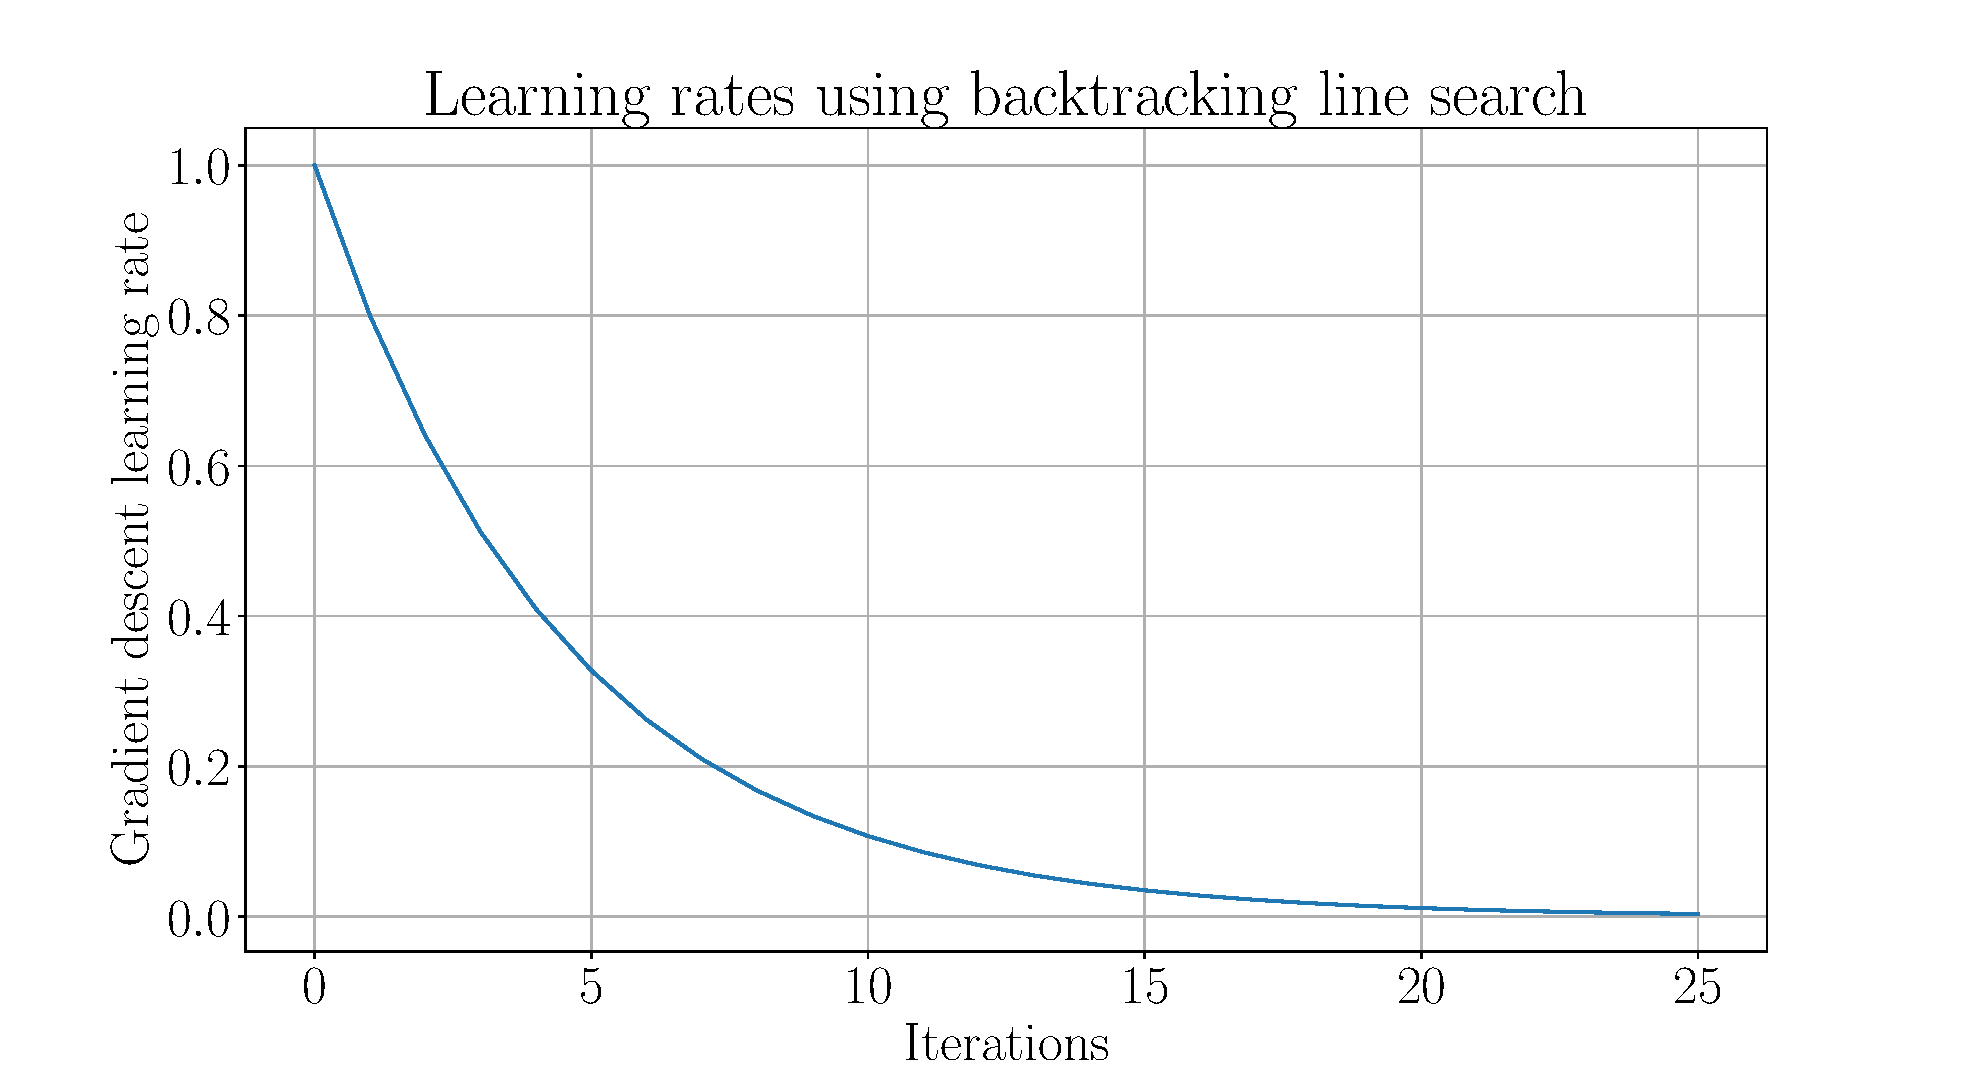
\includegraphics[scale=0.35]{figures/Learning_rates.pdf}}
    \caption[Decay of learning rate for gradient descent optimizer]{\textbf{Decay of learning rate for gradient descent optimizer}: The plot shows how the learning rate for gradient descent evolves with iterations. It start with a small value and decreases gradually over time. It is essential to have learning rates which neither drops too quickly or too slowly.Both of these ways can lead to divergence or slow convergence of the optimizer.}
\end{centering}
\end{figure}

\subsection{Weight update}
\subsubsection{Momentum}
To reach the minimum point of our convex error function (equation 20), we need to go down continously without being blocked at the saddle points. These saddle points are where the derivative of a function is zero. Adding a momentum term to the weight parameter, we expect to avoid the local minima and should be able to converge to the lowest point quickly. It gives the necessary push to keep going down the convex error function by adding the a fraction of the previous step update to the current update \cite{articleRuderS, Sutskever}. We compute the weight parameter update for each iterations using:

\begin{equation}
update_{t+1} = \gamma \cdot update_{t} - \eta \cdot Gradient(w^t)
\end{equation}

\begin{equation}
w_{t+1} = w_t + update_{t+1}
\end{equation}

where $update_{t+1}$ is the update for changing the weight parameter for the current iteration $t+1$. $update_{t-1}$ is previous iteration update. $\eta$ is the learning rate and $Gradient$ is with respect to the weight parameter $w_t$. 

\subsubsection{Nesterov’s accelerated gradient}
The inclusion of momentum is useful to get necessary advance towards finding the minimum of the error function. However, the speed of going down the slope of the error function should become less if there is a possibility of change in gradient direction. In this situation, the speeding up can be avoided by estimating the forthcoming gradient (gradient for the next step) and then correcting it \cite{Botev}. We update the weight parameter using the following equations:

\begin{equation}
update_{t+1} = \gamma \cdot update_t - \eta \cdot Gradient(w_t + \gamma \cdot update_t)
\end{equation}

\begin{equation}
w_{t+1} = w_t + update_{t+1}
\end{equation}

\subsubsection{Gradient verification}
We compute gradient using equation 22 and use it to update our weight parameters. To verify that the computed gradient is correct, we can approximate this gradient using the error function we formulated in equation 20.

\begin{equation}
Gradient(w) = \frac{\partial Error}{\partial w} \approx \frac{Error(w + \epsilon) - Error(w - \epsilon)}{2 \cdot \epsilon} 
\end{equation}
where $\epsilon$ is a very small number. 

\begin{figure}[h]
\begin{centering}
    {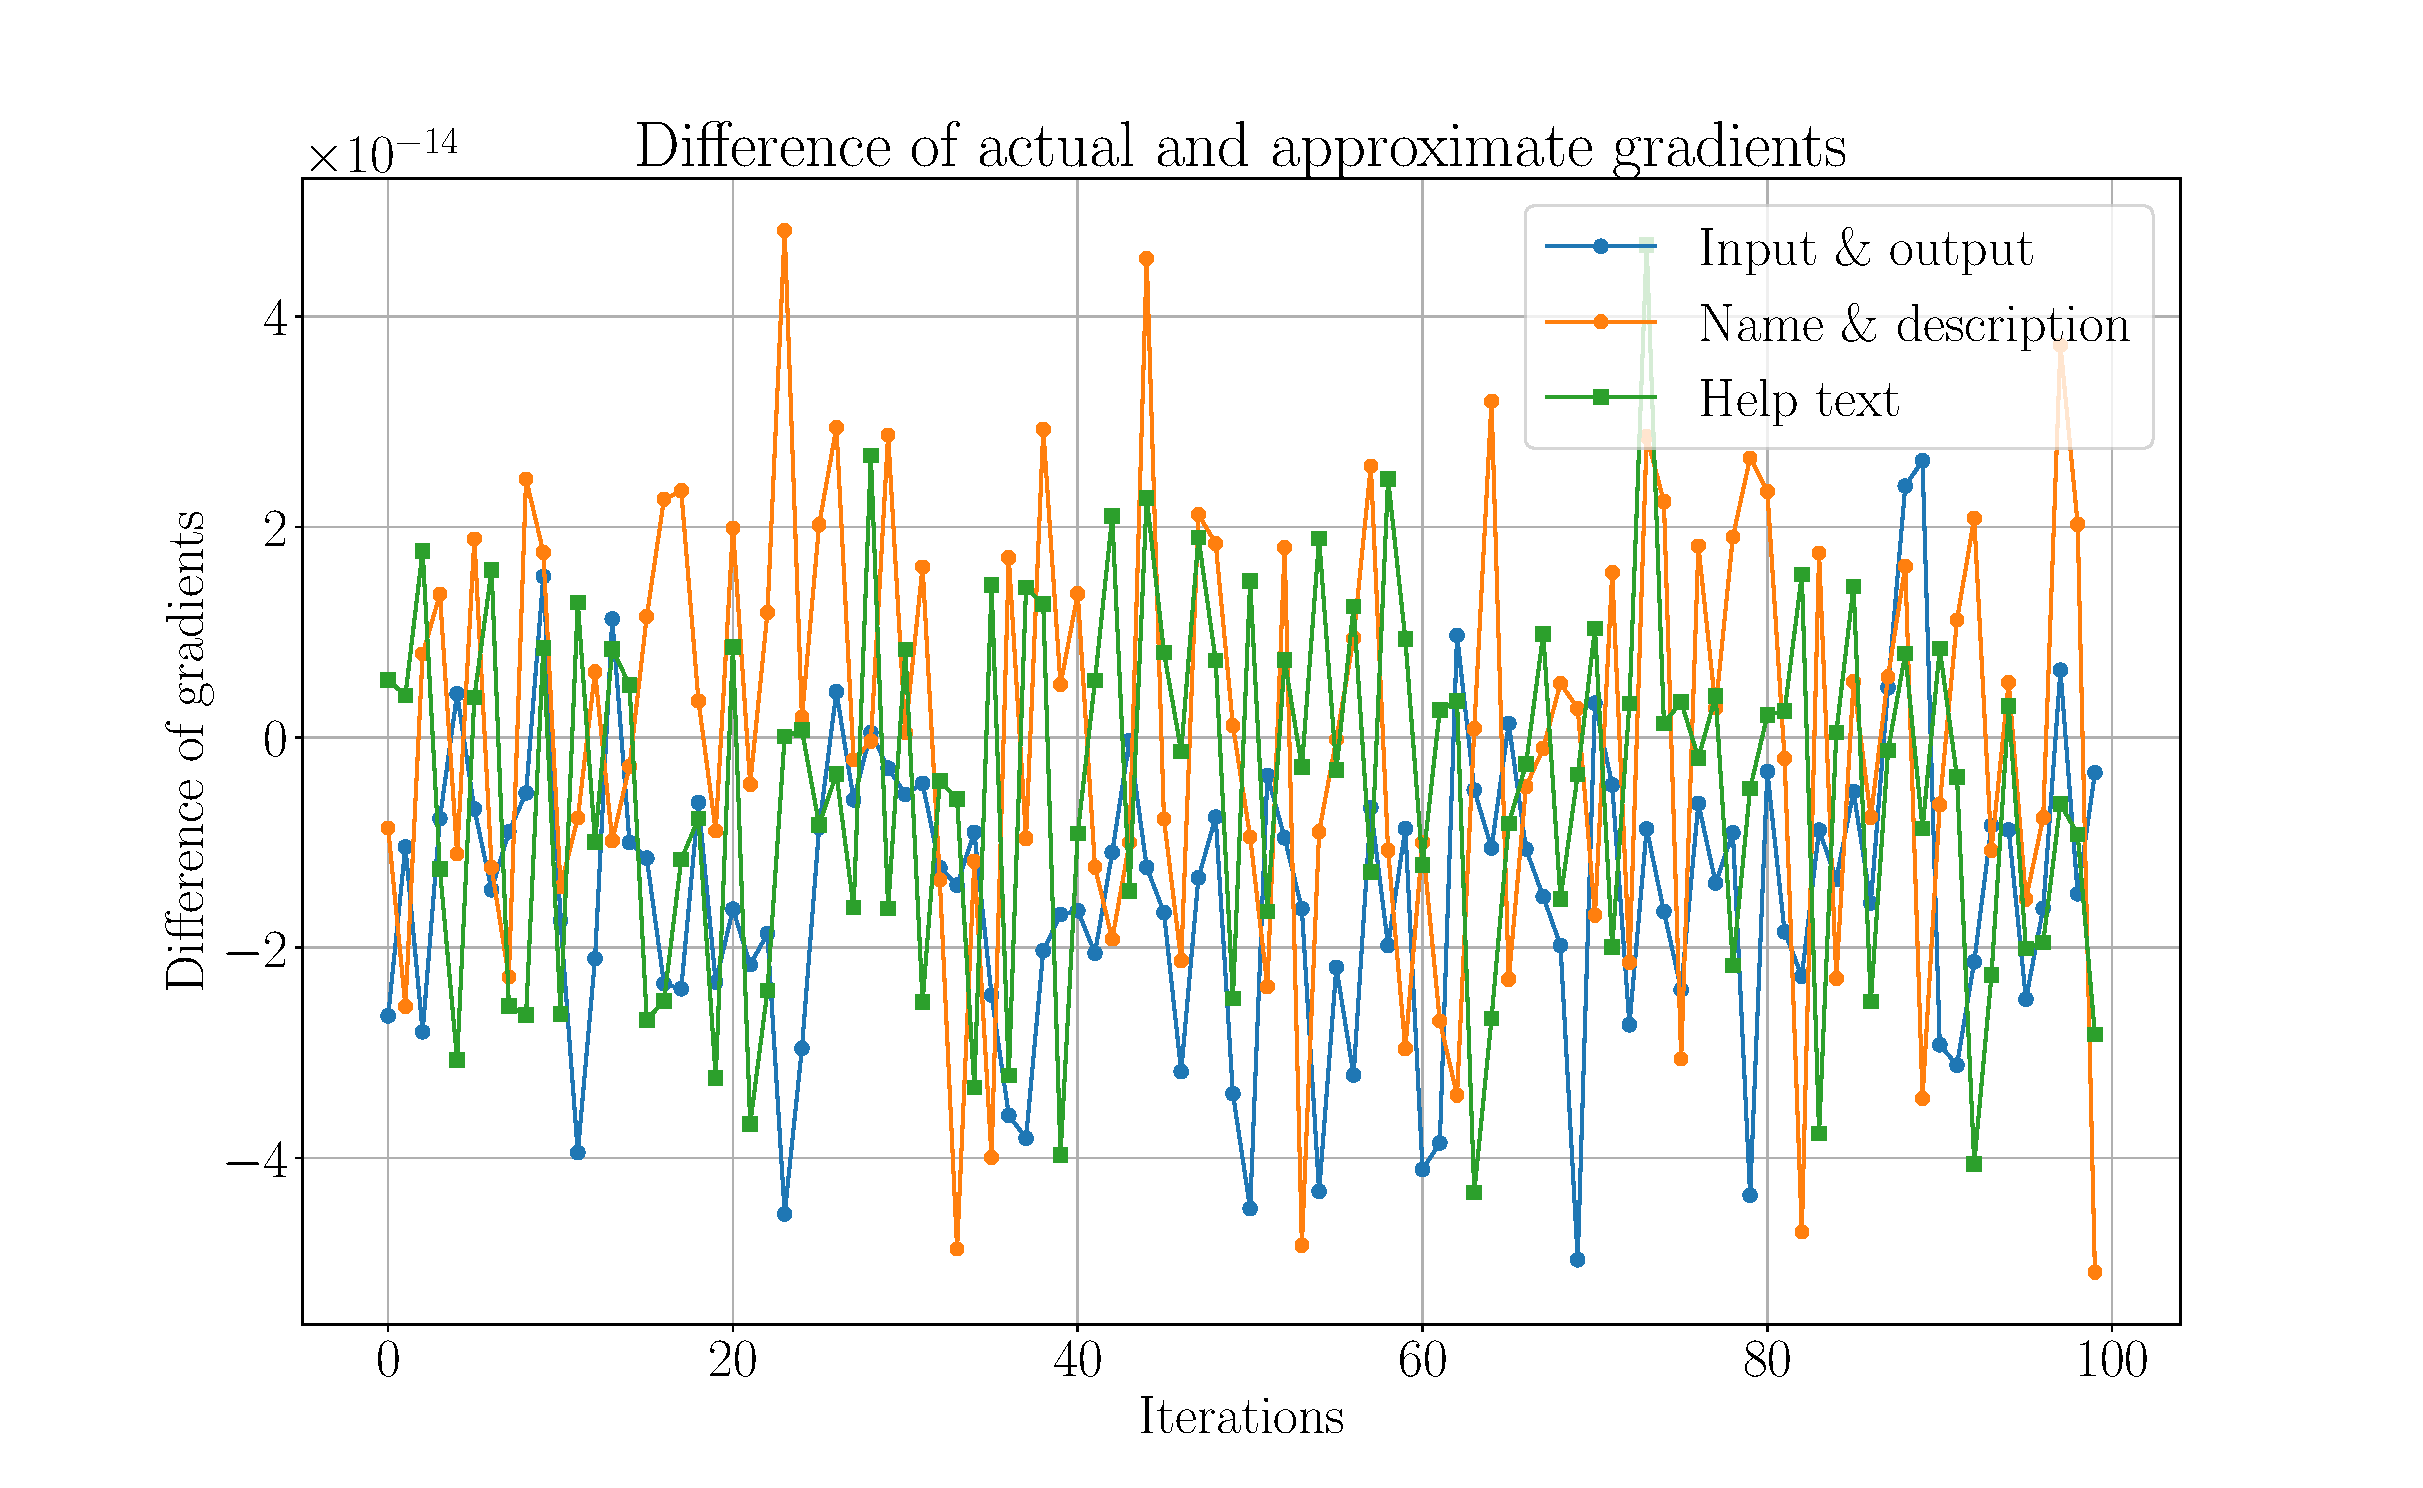
\includegraphics[scale=0.35]{figures/Difference_gradients.pdf}}
    \caption[Verification of gradient for the error function]{\textbf{Verification of gradient for the error function}: The plot checks that the difference between the actual and approximated gradients for all the attributes across all tools computed over 100 iterations is close to 0. Gradient plays an important role in learning and it should be estimated correctly. }
\end{centering}
\end{figure}
